% Sprint 2 — aligné sur la planification (chapitre 2) et le périmètre « Plans & activités » du product backlog
\PFEChapterOpening{Sprint 2 - Gestion des Plans \& activités}

\section{Introduction}
Ce chapitre présente le deuxième sprint du projet, consacré à la mise en place des fonctionnalités liées aux plans CSR et au suivi des activités. Il marque une étape importante en introduisant le cœur fonctionnel de la plateforme, permettant de structurer les données planifiées et réalisées.
Nous y détaillons les besoins identifiés, les choix de conception adoptés ainsi que les modèles UML utilisés. Des interfaces illustrent également les fonctionnalités développées, accompagnées d’une validation permettant de vérifier leur conformité aux attentes.



\section{Objectif attendu}

Ce deuxième sprint a pour finalité de développer le cœur fonctionnel de la plateforme CSR en mettant en place les modules liés à la planification et au suivi des activités. Il vise à permettre aux utilisateurs de définir les plans annuels CSR par site, de renseigner les activités réalisées tout au long de l’année, et d’assurer un suivi structuré et continu de leur exécution. Ce sprint introduit également des mécanismes de comparaison entre le planifié et le réalisé, afin de mesurer les écarts, d’identifier les dépassements budgétaires et d’évaluer le niveau de réalisation des objectifs fixés. Par ailleurs, il intègre la gestion des activités hors plan, offrant ainsi une meilleure maîtrise opérationnelle. L’ensemble de ces fonctionnalités contribue à renforcer la visibilité sur les performances CSR et constitue une étape clé pour l’exploitation future des données à des fins d’analyse décisionnelle.

\section{Sprint Backlog}

Ce sprint est consacré à la gestion des plans CSR et au suivi des activités, en structurant les informations planifiées et réalisées afin d'assurer un pilotage opérationnel clair au niveau des sites.

Le tableau~\ref{tab:sprint-backlog-2} présente le backlog du deuxième sprint.
% --- Sprint backlog — même style visuel que le product backlog (chapitre 2) ---
% Contenu des user stories / tâches 1.x–6.x issu du tableau Word « Tableau 4.1 » ;
% tâches 1.7–1.10 ajoutées pour refléter le cycle plan côté API (soumission, validation, suppression, bulk).
\small
\PFETableSetup

\setlength{\PFEbacklogTabW}{\dimexpr\textwidth+2.8cm\relax}
\setlength{\LTcapwidth}{\PFEbacklogTabW}
\setlength{\LTleft}{\fill}
\setlength{\LTright}{\fill}

\setlength{\LTpre}{0pt}
\setlength{\LTpost}{0pt}

\PFETableArrayStretch
\setlength{\extrarowheight}{4pt}
\renewcommand{\arraystretch}{1.4}

\arrayrulecolor{black}

\begin{longtable}{|
>{\centering\arraybackslash}m{1.2cm}|
>{\raggedright\arraybackslash}m{5.2cm}|
>{\centering\arraybackslash}m{1.6cm}|
>{\raggedright\arraybackslash}m{5.5cm}|
>{\centering\arraybackslash}m{1.7cm}|}

\caption{Sprint backlog du sprint 2 — Plans \& activités}\label{tab:sprint-backlog-2}\\

\hline
\tableHeaderStyle
\tableHeaderCell{ID} & \tableHeaderCell{User story} & \tableHeaderCell{Tâche ID} & \tableHeaderCell{Tâche} & \tableHeaderCell{Priorité} \\
\hline
\endfirsthead

\hline
\multicolumn{5}{|c|}{\tablename\ \thetable{} — \textit{(suite)}} \\
\hline
\tableHeaderStyle
\tableHeaderCell{ID} & \tableHeaderCell{User story} & \tableHeaderCell{Tâche ID} & \tableHeaderCell{Tâche} & \tableHeaderCell{Priorité} \\
\hline
\endhead

\hline
\multicolumn{5}{|r|}{\textit{Suite page suivante\ldots}} \\
\hline
\endfoot

\hline
\endlastfoot

1 & En tant qu'utilisateur (Site ou Corporate), je veux créer un plan CSR afin de planifier les activités & 1.1 &
Implémenter le module de gestion des plans CSR & +++++ \\
\cline{3-5}
& & 1.2 &
Permettre à l'utilisateur site de créer un plan CSR pour les sites auxquels il est rattaché & +++++ \\
\cline{3-5}
& & 1.3 &
Permettre à l'utilisateur corporate de créer un plan CSR à l'échelle de tous les sites & +++++ \\
\cline{3-5}
& & 1.4 &
Définir les informations du plan (site, année, budget total, \ldots) & +++++ \\
\cline{3-5}
& & 1.5 &
Modifier un plan CSR avant validation & ++++ \\
\cline{3-5}
& & 1.6 &
Consulter les plans CSR par année / statut / site & +++ \\
\cline{3-5}
& & 1.7 &
Soumettre un plan CSR pour validation (passage au statut soumis) & +++++ \\
\cline{3-5}
& & 1.8 &
Permettre à l'utilisateur corporate de valider ou de rejeter un plan soumis avec motif & +++++ \\
\cline{3-5}
& & 1.9 &
Supprimer un plan CSR lorsque les règles métier le permettent & ++++ \\
\cline{3-5}
& & 1.10 &
Soumettre ou supprimer plusieurs plans en une seule opération (actions en masse) & ++++ \\
\cline{3-5}
& & 1.11 &
Rechercher un plan CSR (par mot-clé, site, année) & ++++ \\
\cline{3-5}
& & 1.12 &
Filtrer les plans CSR selon des critères (statut, site, année) & ++++ \\
\cline{3-5}
& & 1.13 &
Soumettre une demande de modification sur un plan verrouillé & ++++ \\
\hline
2 & En tant qu'utilisateur, je veux importer un plan CSR via un fichier Excel afin de gagner du temps & 2.1 &
Implémenter la fonctionnalité d'import Excel & +++++ \\
\cline{3-5}
& & 2.2 &
Lire et parser le fichier Excel avant l'importer & +++++ \\
\cline{3-5}
& & 2.3 &
Valider les données (site, année, mode de validation) pour l'utilisateur site & +++++ \\
\cline{3-5}
& & 2.4 &
Détecter les conflits (doublons, incohérences) & +++++ \\
\cline{3-5}
& & 2.5 &
Afficher un aperçu avant l'importer & ++++ \\
\cline{3-5}
& & 2.6 &
Supprimer les duplicatas avant la validation & ++++ \\
\cline{3-5}
& & 2.7 &
Ignorer les duplicatas et continuer avant la validation & ++++ \\
\hline
3 & En tant qu'utilisateur Site, je veux gérer les activités planifiées afin d'organiser les actions CSR & 3.1 &
Ajouter une méthode pour ajouter activité planifiée & +++++ \\
\cline{3-5}
& & 3.2 &
Ajouter les informations nécessaires de chaque activité planifiée(titre,numéro, catégorie, budget prévu, Impact de l'action prévue \ldots) & +++++ \\
\cline{3-5}
& & 3.3 &
Ajouter une méthode de  modification de l'activité planifiée avant validation & ++++ \\
\cline{3-5}
& & 3.4 &
Ajouter une méthode de suppression de l'activité planifiée avant validation & ++++ \\
\cline{3-5}
& & 3.5 &
Ajouter une méthode de consultation du détail d'une activité planifiée & ++++ \\
\cline{3-5}
& & 3.6 &
Ajouter une fonctionnalité de recherche des activités planifiées & ++++ \\
\cline{3-5}
& & 3.7 &
Ajouter une fonctionnalité de filtrage des activités planifiées & ++++ \\
\hline
4 & En tant qu'utilisateur Site, je veux saisir les activités réalisées afin de suivre l'exécution & 4.1 &
Implémenter le module des activités réalisées & +++++ \\
\cline{3-5}
& & 4.2 &
Ajouter une méthode pour saisir  les données de l'activité réalisée( Budget réalisé, participants, Date de réalisation, \ldots) & +++++ \\
\cline{3-5}
& & 4.3 &
Ajouter une méthode de  modification de l'activité réalisée & ++++ \\
\cline{3-5}
& & 4.4 &
Ajouter une méthode de suppression de l'activité réalisée & ++++ \\
\cline{3-5}
& & 4.5 &
Ajouter une méthode de consultation du détail d'une activité réalisée & ++++ \\
\cline{3-5}
& & 4.6 &
Ajouter une fonctionnalité de recherche des activités réalisées & ++++ \\
\cline{3-5}
& & 4.7 &
Ajouter une fonctionnalité de filtrage des activités réalisées & ++++ \\
\hline
5 & En tant qu'utilisateur Site, je veux ajouter des activités hors plan afin de tracer les actions imprévues & 5.1 &
Ajouter une méthode de création d'une activité hors plan & +++++ \\
\cline{3-5}
& & 5.2 &
Saisir toutes les informations de l'activité hors plan (titre, catégorie, date de réalisation, \ldots) & +++++ \\
\cline{3-5}
& & 5.3 &
Ajouter une méthode de  modification de l'activité hors plan & ++++ \\
\cline{3-5}
& & 5.4 &
Ajouter une méthode de suppression de l'activité hors plan & ++++ \\
\cline{3-5}
& & 5.5 &
Soumettre une activité hors plan pour validation & ++++ \\
\hline
6 & En tant qu'utilisateur, je veux visualiser les informations planifiées et réalisées afin d'avoir une vue complète & 6.1 &
Afficher les données planifiées( Budget prévu, impact prévu de l'action, nombre de participants prévus, \ldots) & +++++ \\
\cline{3-5}
& & 6.2 &
Afficher les données réalisées( Budget réalisé, impact de l'action , nombre réel de participants, \ldots) & +++++ \\
\hline

\end{longtable}

\normalsize

\newpage
\section{Analyse détaillée des besoins}

\subsection{Diagramme de cas d'utilisation}

La figure~\ref{fig:doc-ch4-1} illustre le diagramme de cas d'utilisation du deuxième sprint.

\IfFileExists{figures/chapitre-04/diagramme-cas-utilisation-plans-activites.png}{%
\begin{figure}[H]
  \centering
  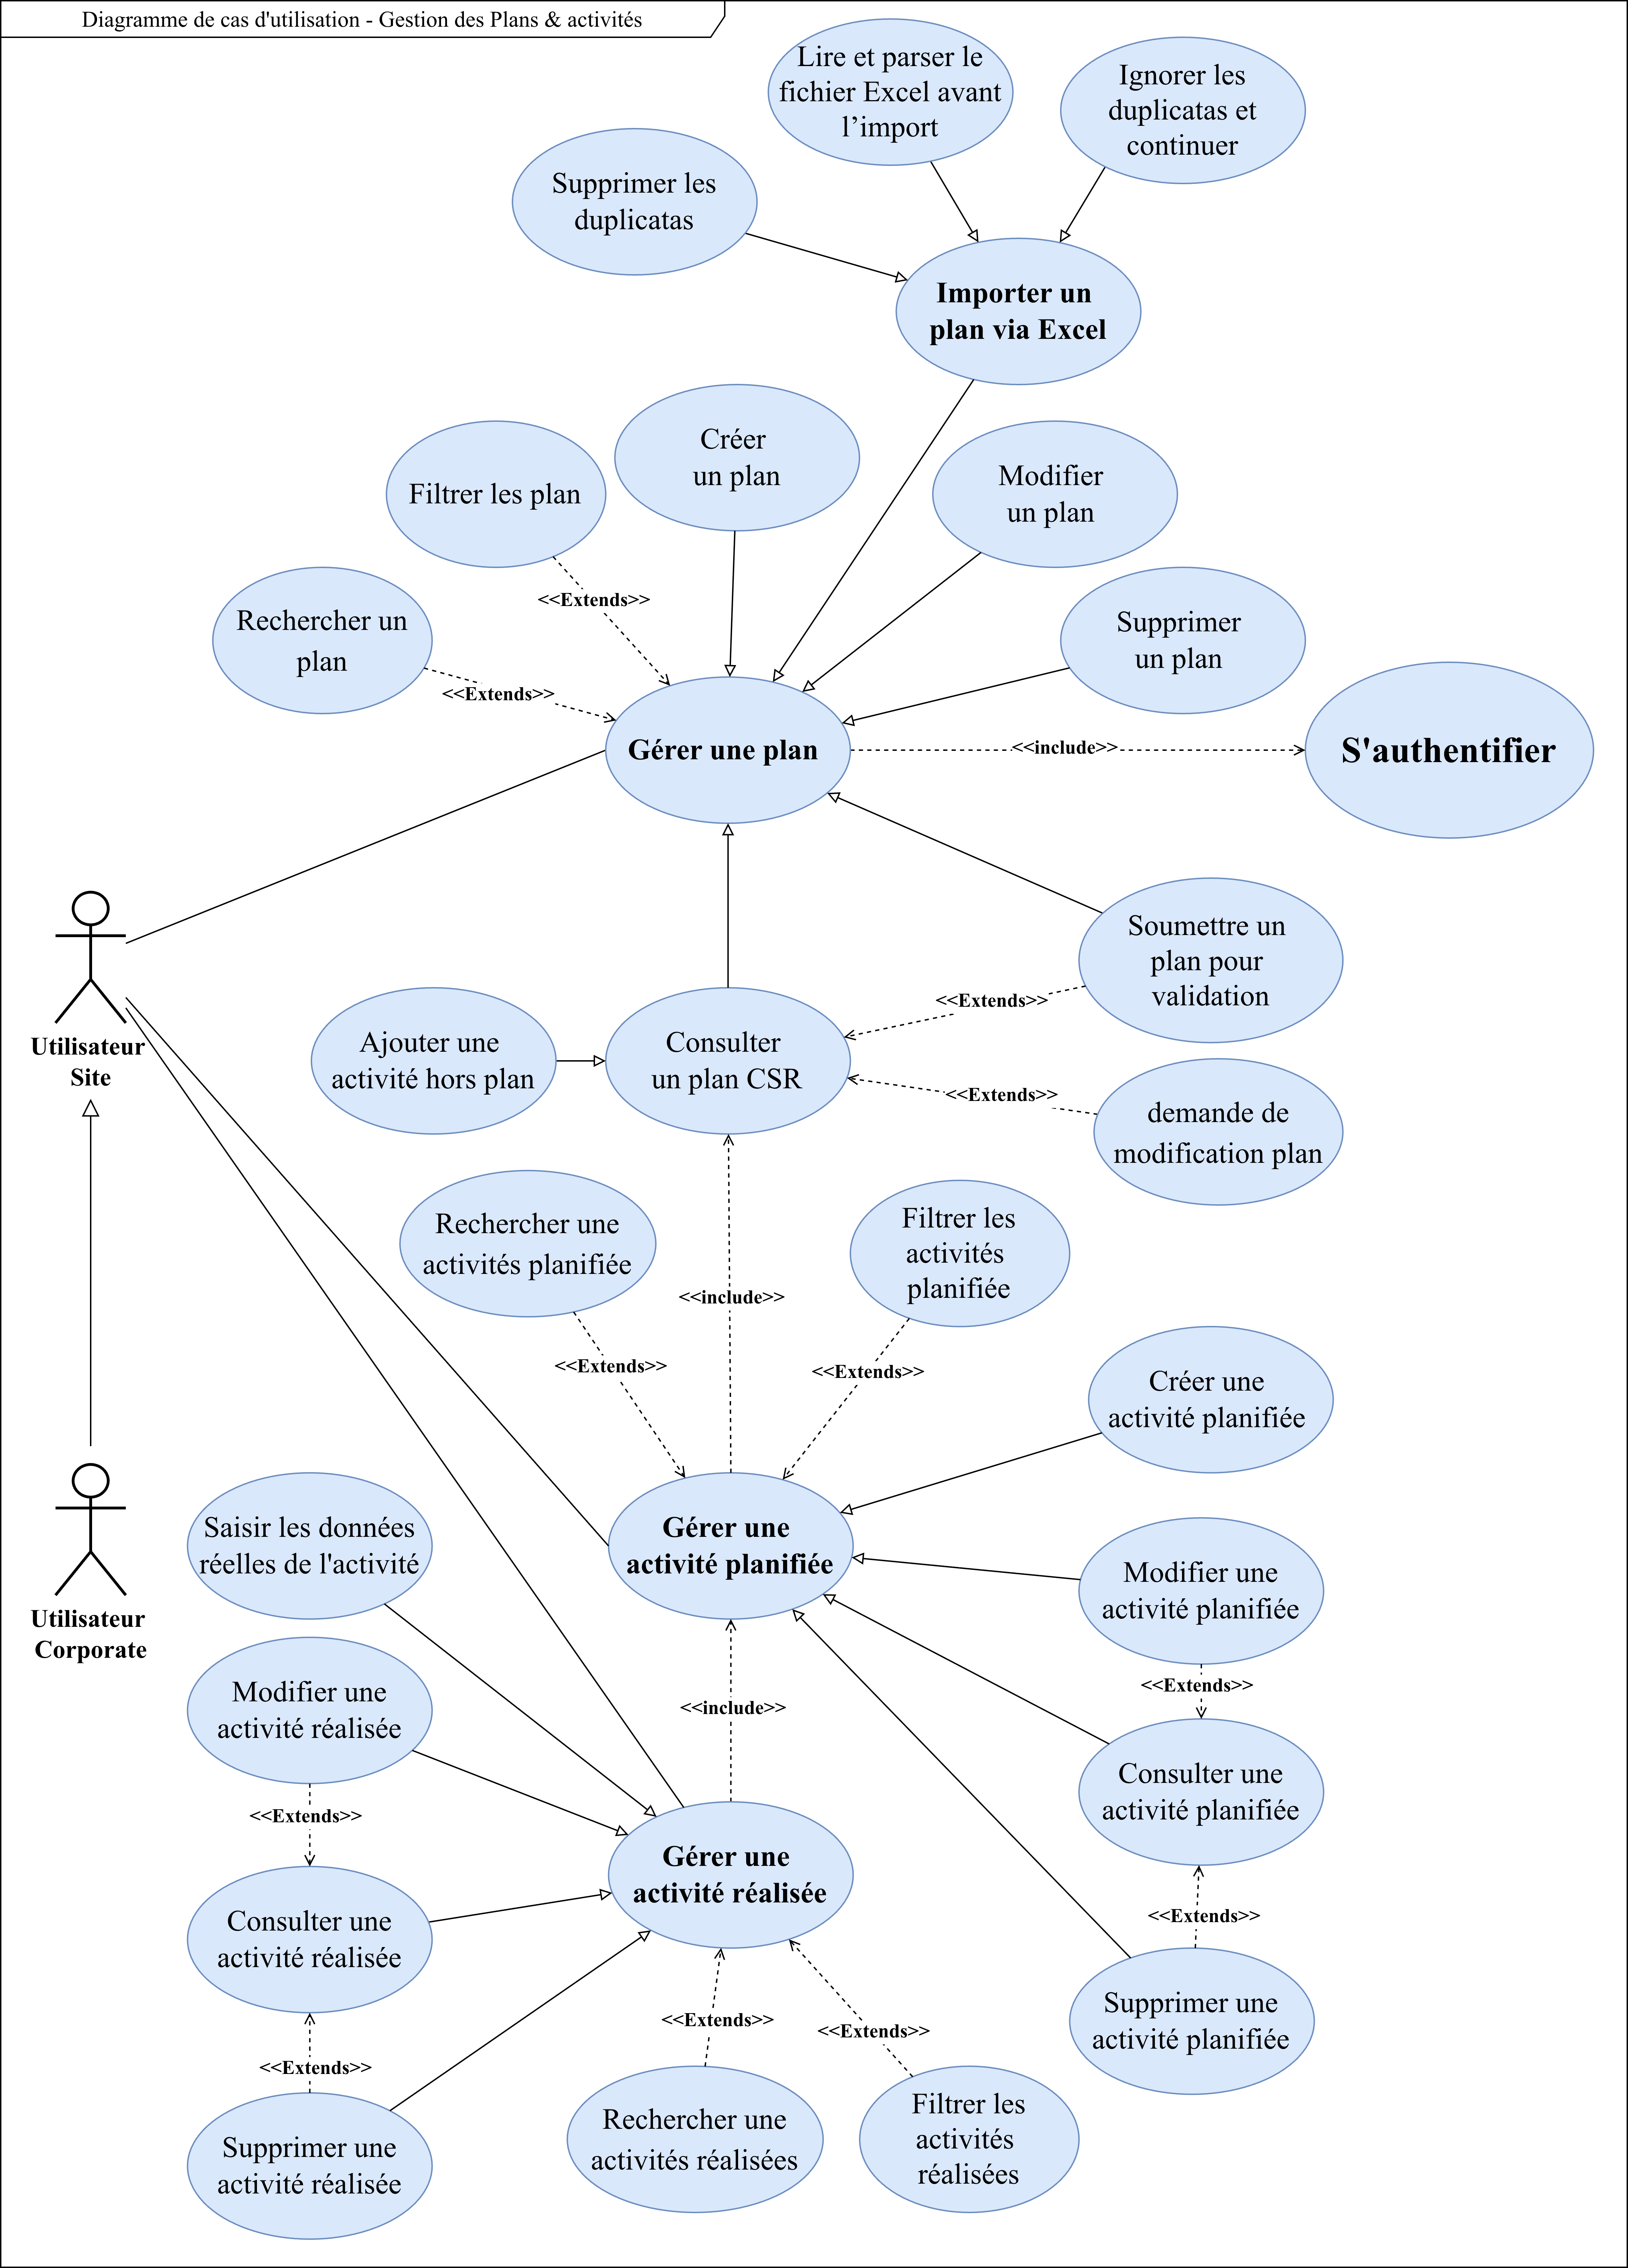
\includegraphics[width=0.92\linewidth]{figures/chapitre-04/diagramme-cas-utilisation-plans-activites.png}
  \caption{Diagramme de cas d'utilisation du deuxième sprint.}
  \label{fig:doc-ch4-1}
\end{figure}%
}{%
\begin{figure}[H]
  \centering
  \fbox{\parbox{0.92\linewidth}{\centering\vspace{3.2cm}\textit{(Figure à insérer : \texttt{figures/chapitre-04/diagramme-cas-utilisation-plans-activites.png})}\vspace{3.2cm}}}
  \caption{Diagramme de cas d'utilisation du deuxième sprint.}
  \label{fig:doc-ch4-1}
\end{figure}%
}
\newpage

\subsection{Description textuelle du cas d'utilisation : «~Créer un plan CSR~»}

Le tableau~\ref{tab:cu-creer-plan-csr} expose la description textuelle du cas d'utilisation «~Créer un plan CSR~».

% Cas d'utilisation « Créer un plan CSR » — inclus sous la sous-section 4.4.2
\begin{table}[H]
  \centering
  \small
  \caption{Description textuelle du cas d'utilisation : «~Créer un plan CSR~»}
  \label{tab:cu-creer-plan-csr}
  \PFETableSetup
  \PFETableRowColors
  \PFETableArrayStretch
  \PFETableTabularXBegin
  \begin{tabularx}{\PFETableBlockWidth}{@{}>{\raggedright\arraybackslash}p{3.2cm} >{\raggedright\arraybackslash}X@{}}
    \tableHeaderStyle \tableHeaderCell{Champ} & \tableHeaderCell{Contenu} \\
    \textbf{Titre} & Créer un plan CSR \\
    \textbf{Acteurs} & Utilisateur Corporate ; utilisateur Site. \\
    \textbf{Objectif} &
      Permettre aux utilisateurs de définir un plan CSR annuel afin de structurer la planification des activités et organiser les initiatives au niveau des sites. \\
    \textbf{Préconditions} &
      1. L'utilisateur est authentifié.\par
      2. Un token est obtenu pour accéder aux ressources protégées. \\
    \textbf{Postconditions} &
      1. Les informations du plan (site, année, budget, etc.) sont sauvegardées.\par
      2. Le plan devient disponible pour l'ajout des activités. \\
    \textbf{Scénario nominal} &
      1. L'utilisateur accède au module des plans CSR.\par
      2. Le système affiche les plans existants.\par
      3. L'utilisateur sélectionne l'option de création d'un plan.\par
      4. Il saisit les informations du plan (site(s), année, budget total, etc.).\par
      5. Le système vérifie la validité des données.\par
      6. Le système enregistre le plan CSR.\par
      7. Le plan apparaît dans la liste des plans disponibles. \\
    \textbf{Scénario alternatif} &
      \textbf{A. Plan déjà existant :} \par
      A.1 L'utilisateur tente de créer un plan pour un site et une année déjà existants. \par
      A.2 Le système rejette l'opération. \par
      A.3 Un message est affiché : «~Un plan existe déjà pour ce site et cette année~». \par\medskip
      \textbf{B. Données invalides :} \par
      B.1 L'utilisateur saisit des informations incomplètes. \par
      B.2 Le système bloque la création du plan. \par
      B.3 Un message d'erreur s'affiche en fonction des informations manquantes. \\
  \end{tabularx}%
  \PFETableTabularXEnd
\end{table}

\newpage

\subsection{Description textuelle du cas d'utilisation : «~Soumettre un plan CSR pour validation~»}

Le tableau~\ref{tab:cu-soumettre-plan-csr} expose la description textuelle du cas d'utilisation «~Soumettre un plan CSR pour validation~».

% Cas d'utilisation « Soumettre un plan CSR pour validation » — inclus sous la sous-section 4.4.3
\begin{table}[H]
  \centering
  \small
  \caption{Description textuelle du cas d'utilisation : «~Soumettre un plan CSR pour validation~»}
  \label{tab:cu-soumettre-plan-csr}
  \PFETableSetup
  \PFETableRowColors
  \PFETableArrayStretch
  \PFETableTabularXBegin
  \begin{tabularx}{\PFETableBlockWidth}{@{}>{\raggedright\arraybackslash}p{3.2cm} >{\raggedright\arraybackslash}X@{}}
    \tableHeaderStyle \tableHeaderCell{Champ} & \tableHeaderCell{Contenu} \\
    \textbf{Titre} & Soumettre un plan CSR pour validation \\
    \textbf{Acteurs} & Utilisateur Corporate ; utilisateur Site. \\
    \textbf{Objectif} &
      Permettre à l'utilisateur de soumettre un plan CSR afin de lancer le processus de validation et de figer les informations avant son exécution. \\
    \textbf{Préconditions} &
      1. L'utilisateur est authentifié.\par
      2. Un token est obtenu pour accéder aux ressources protégées.\par
      3. Un plan CSR existe.\par
      4. Le plan est complet et en état modifiable. \\
    \textbf{Postconditions} &
      1. Le plan CSR passe à l'état «~soumis~».\par
      2. Il devient non modifiable selon les règles métier.\par
      3. Il est prêt pour le processus de validation.\par
      4. Une notification est envoyée à l'utilisateur corporate. \\
    \textbf{Scénario nominal} &
      1. L'utilisateur accède au module des plans CSR.\par
      2. Le système affiche la liste des plans existants.\par
      3. L'utilisateur sélectionne un plan.\par
      4. Le système affiche les détails du plan.\par
      5. L'utilisateur déclenche l'action de soumission.\par
      6. Le système vérifie que les informations requises sont complètes.\par
      7. Le système change le statut du plan en «~soumis~».\par
      8. Le système enregistre la modification. \\
    \textbf{Scénario alternatif} &
      \textbf{A. Données incomplètes :} \par
      A.1 Le système refuse la soumission. \par
      A.2 Il signale les champs ou règles non satisfaits. \par\medskip
      \textbf{B. Plan non modifiable :} \par
      B.1 Le système informe l'utilisateur que la soumission n'est pas possible. \par
      B.2 Le message indique la cause (statut, droits ou fenêtre de modification). \\
  \end{tabularx}%
  \PFETableTabularXEnd
\end{table}


\section{Modélisation conceptuelle}

Dans cette section, nous détaillons les choix de conception adoptés pour le \textbf{deuxième sprint}. Nous y présentons d'abord le diagramme de classes, puis nous illustrons les principaux cas d'utilisation à travers des diagrammes de séquence, afin d'expliciter les interactions entre les composants du système.

\subsection{Diagramme de classe}


La figure~\ref{fig:doc-ch4-2} représente le diagramme de classe du deuxième sprint.

\begin{figure}[H]
  \centering
  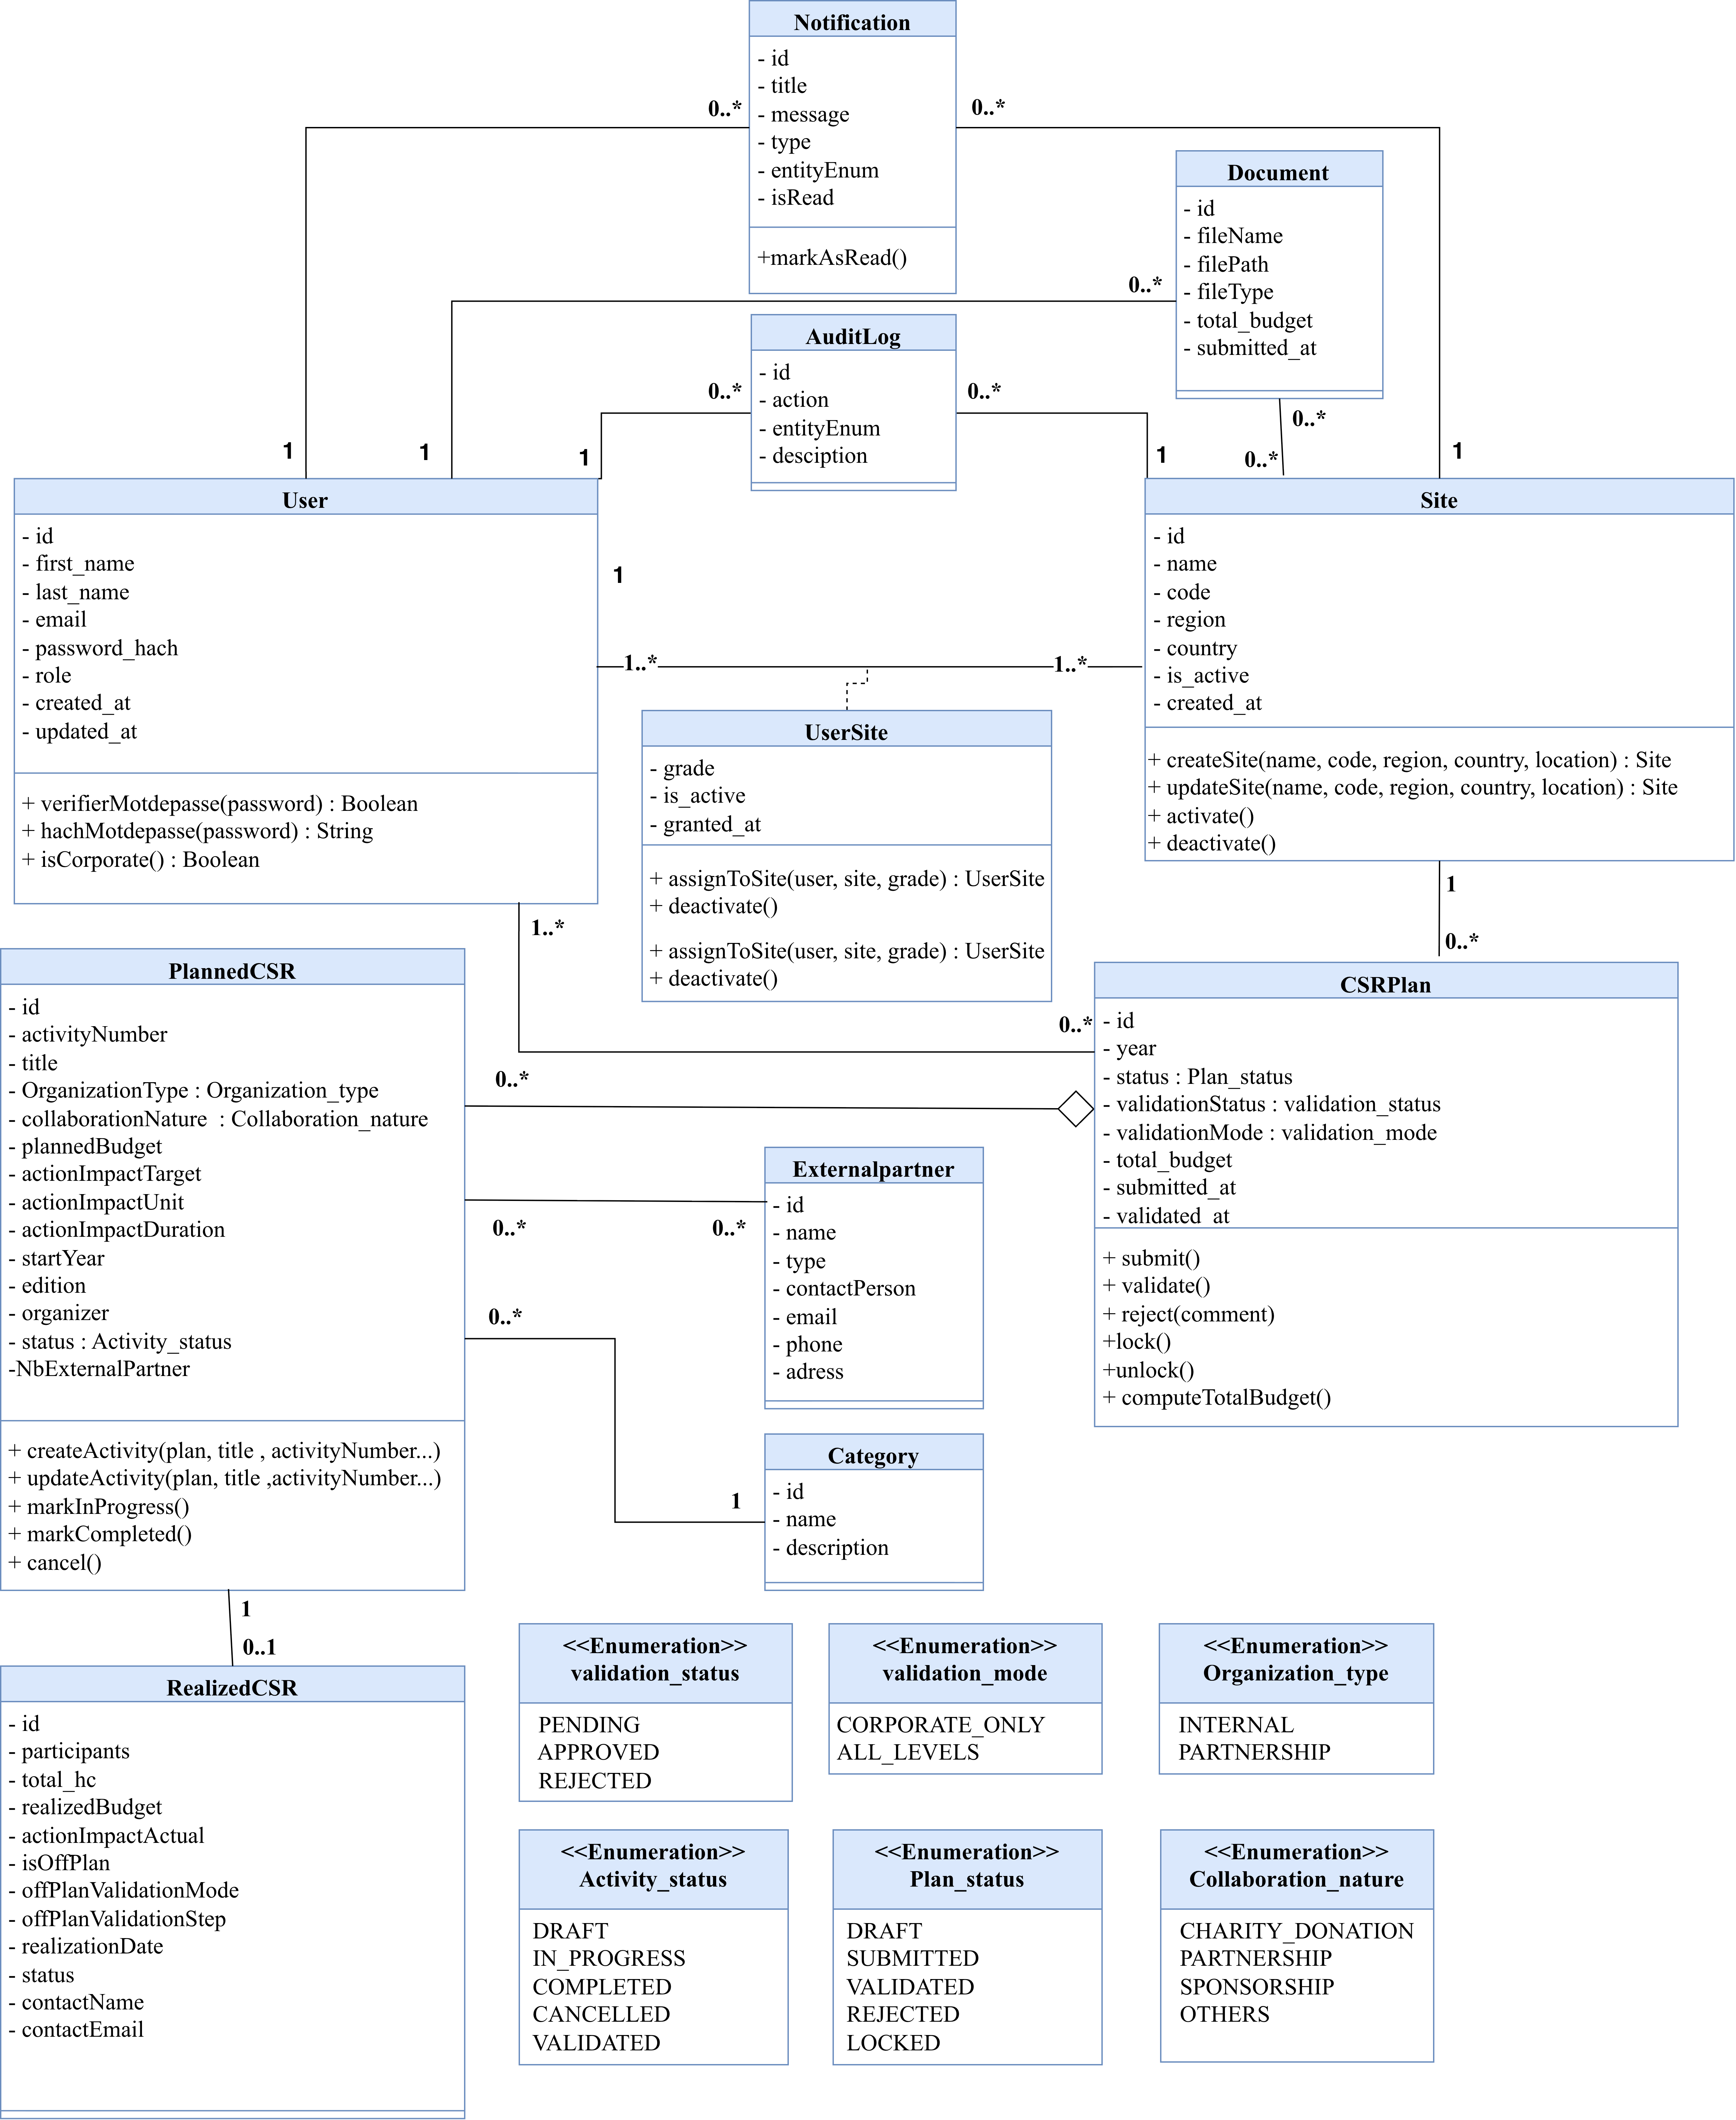
\includegraphics[width=0.82\linewidth]{figures/chapitre-04/diagramme-classe-plans-activites.png}
  \caption{Diagramme de classe -- Gestion des plans \& activités.}
  \label{fig:doc-ch4-2}
\end{figure}%


\subsection{Diagramme de séquence}

Les diagrammes de séquence décrivent les interactions dynamiques entre les composants du système. Nous détaillons ici deux scénarios essentiels du sprint~: la \textbf{création d'un plan CSR} et la \textbf{modification d'une activité planifiée}.        

\subsubsection{Diagramme de séquence : «~Créer un plan CSR~»}

La figure~\ref{fig:doc-ch4-seq-creer-plan} présente le scénario «~Créer un plan CSR~».

\begin{figure}[H]
  \centering
  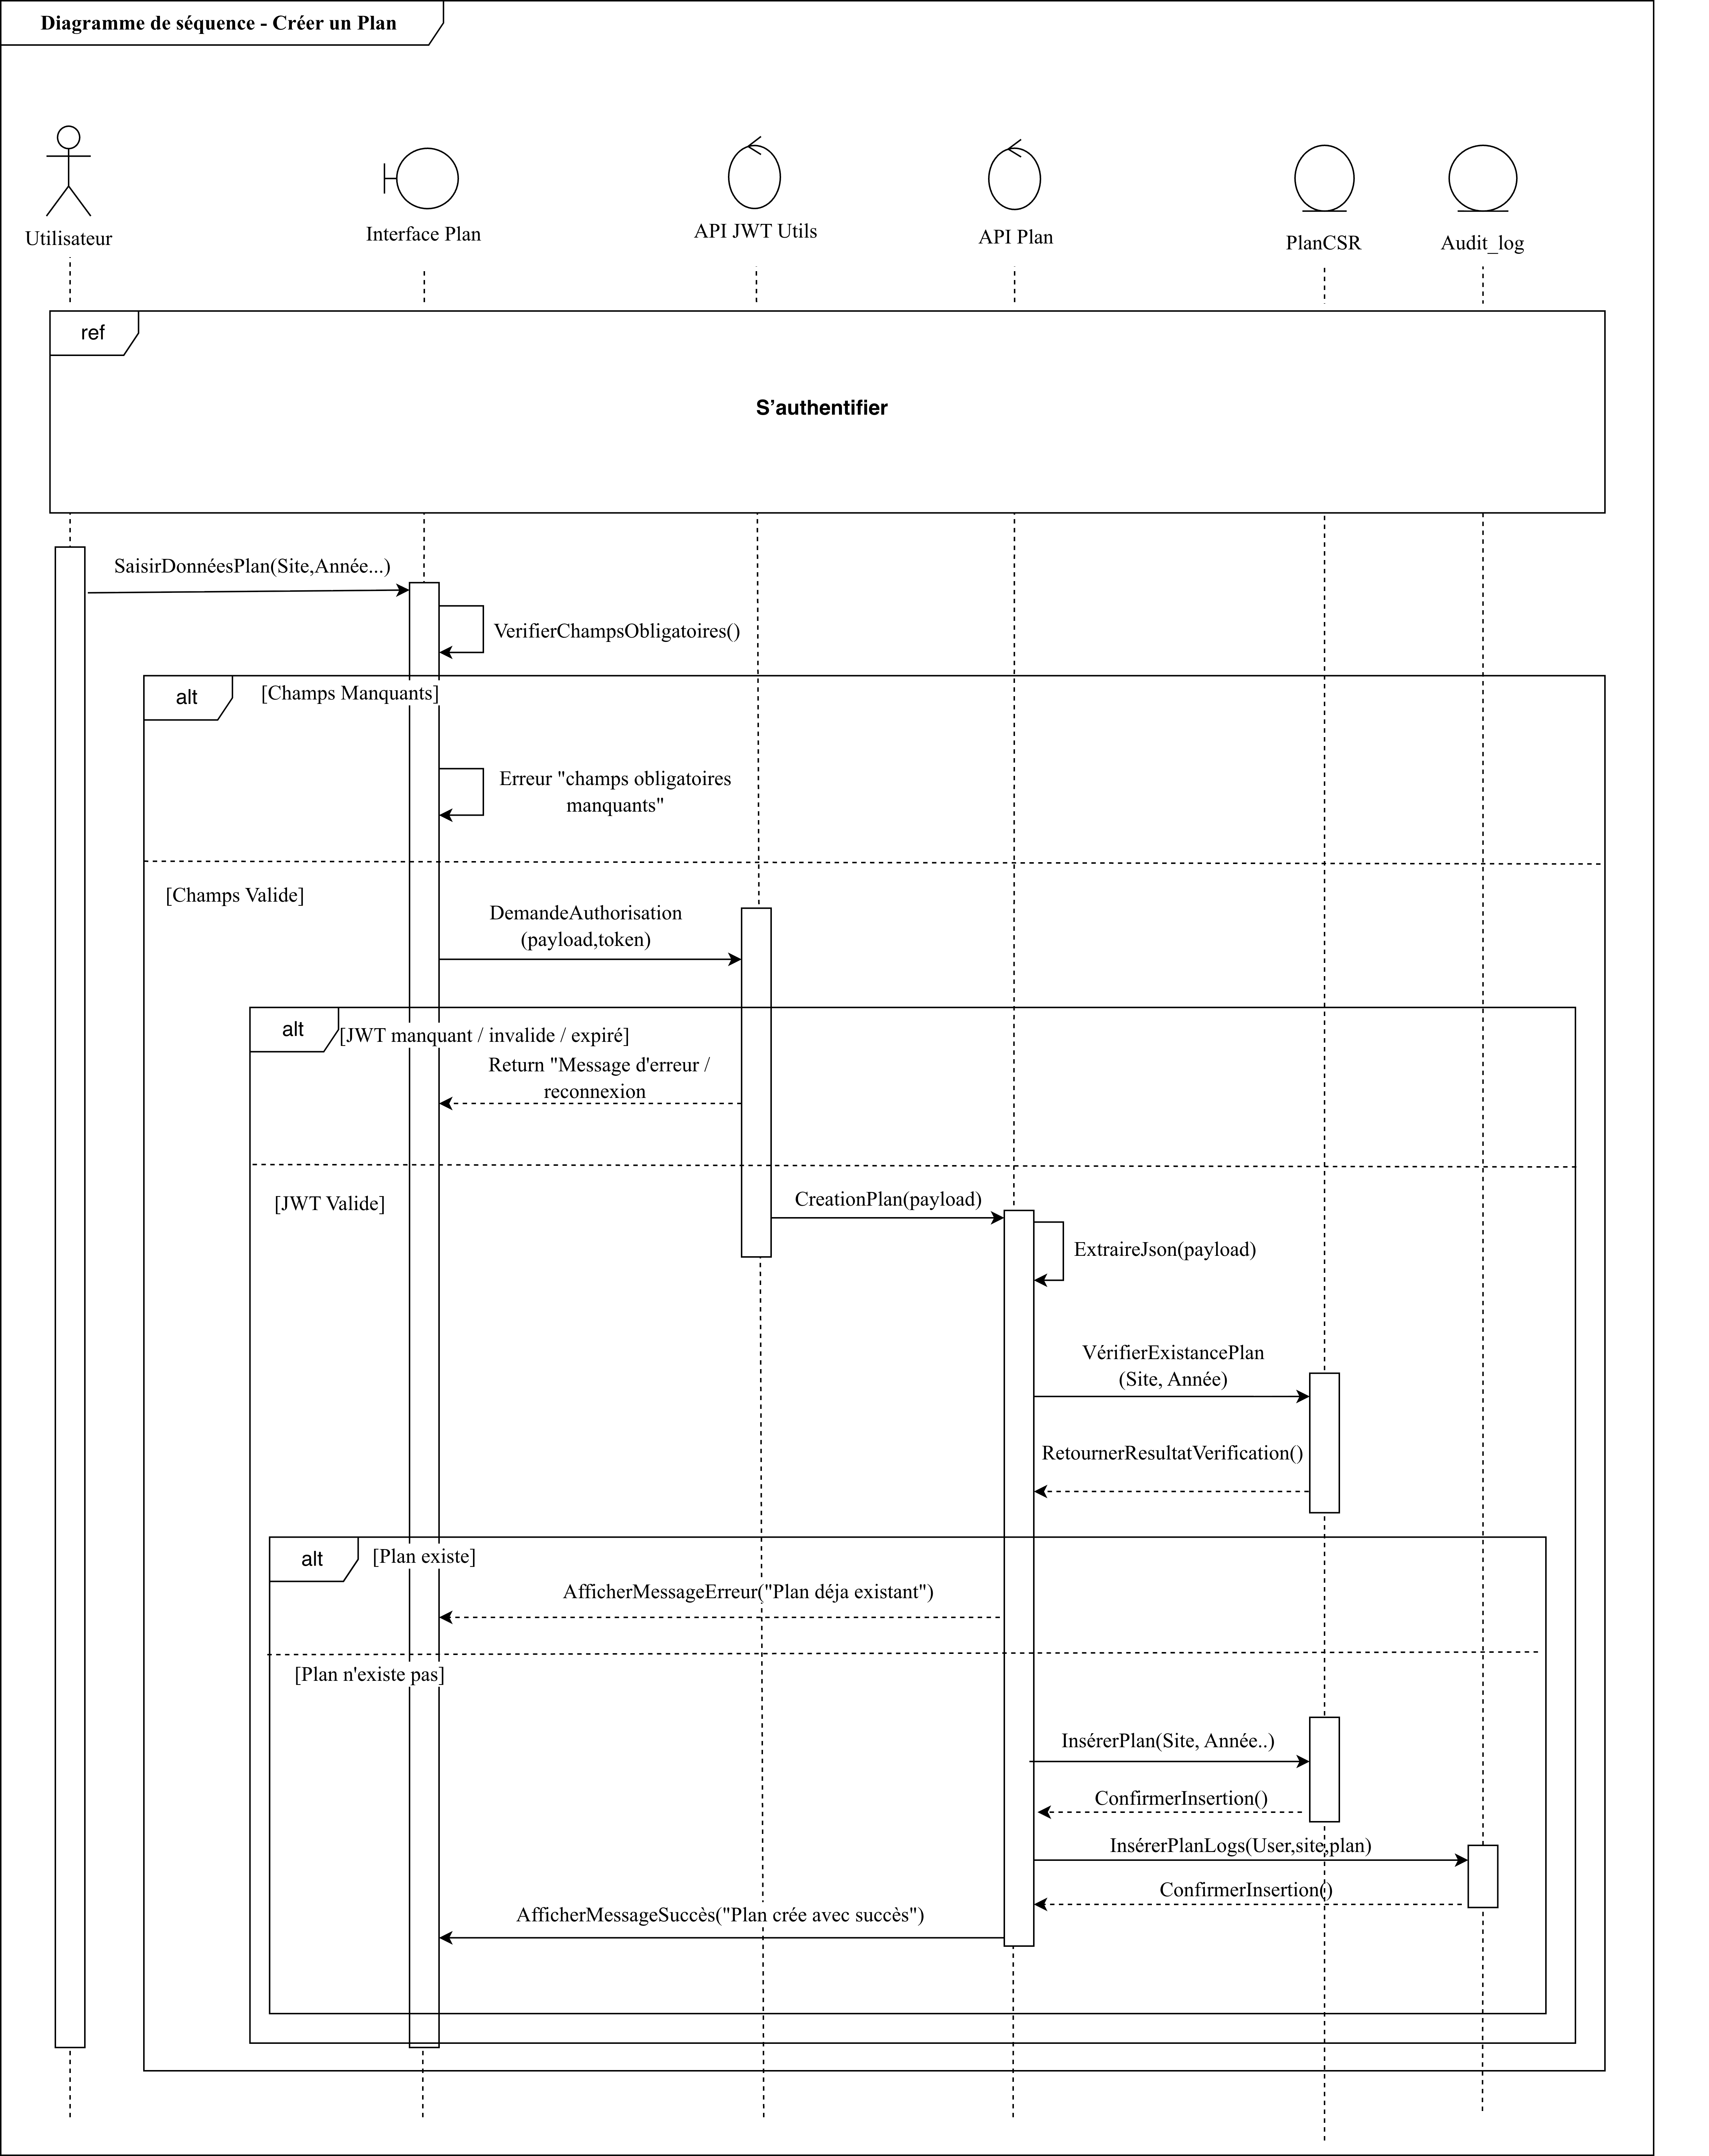
\includegraphics[width=0.92\linewidth]{figures/chapitre-04/diagramme-sequence-creer-plan-csr.png}
  \caption{Diagramme de séquence — «~Créer un plan CSR~».}
  \label{fig:doc-ch4-seq-creer-plan}
\end{figure}

\subsubsection{Diagramme de séquence : «~Modifier une activité planifiée~»}

La figure~\ref{fig:doc-ch4-seq-modif-activite} présente le scénario «~Modifier une activité planifiée~».

\begin{figure}[H]
  \centering
  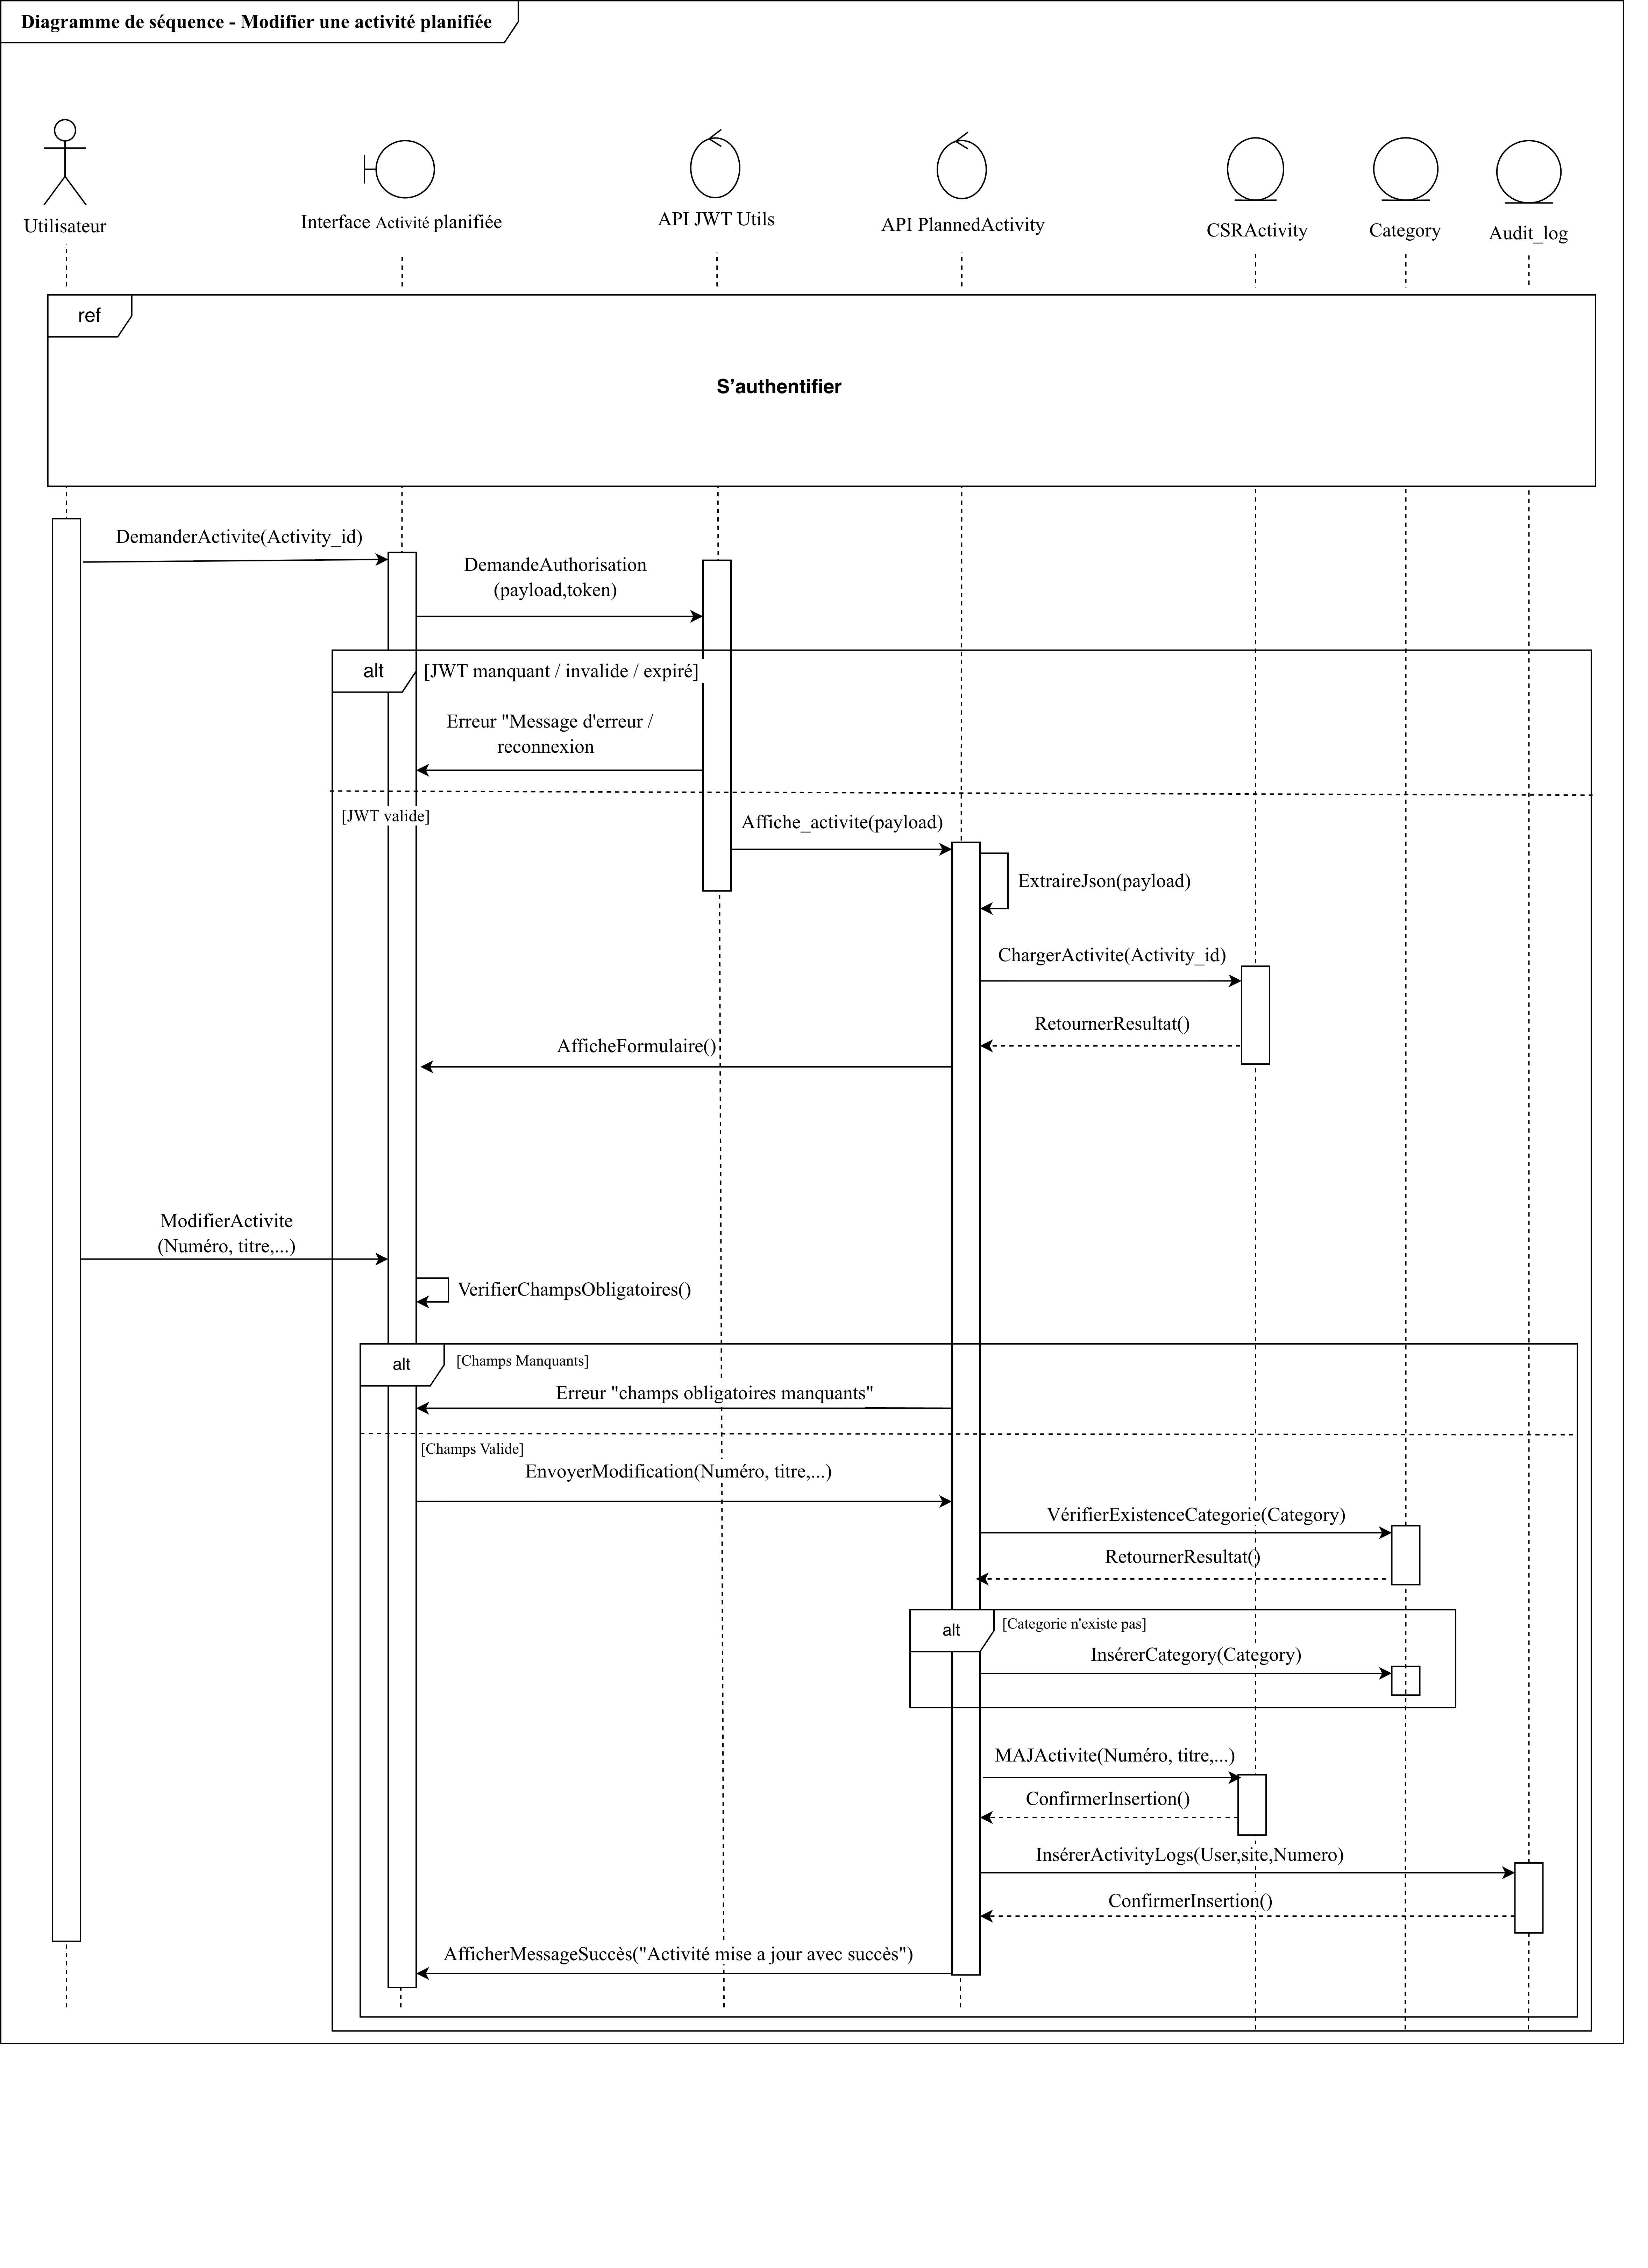
\includegraphics[width=0.92\linewidth]{figures/chapitre-04/diagramme-sequence-modifier-activite-planifiee.png}
  \caption{Diagramme de séquence — «~Modifier une activité planifiée~».}
  \label{fig:doc-ch4-seq-modif-activite}
\end{figure}%

\subsection{Diagramme d’activité}

Les diagrammes d’activité présentent l’enchaînement des traitements et des décisions métier pour les fonctionnalités clés du sprint 2.

\subsubsection{Diagramme d’activité : «~Créer un plan CSR~»}

La figure~\ref{fig:doc-ch4-act-creer-plan} présente le diagramme d’activité du cas «~Créer un plan CSR~».

\begin{figure}[H]
  \centering
  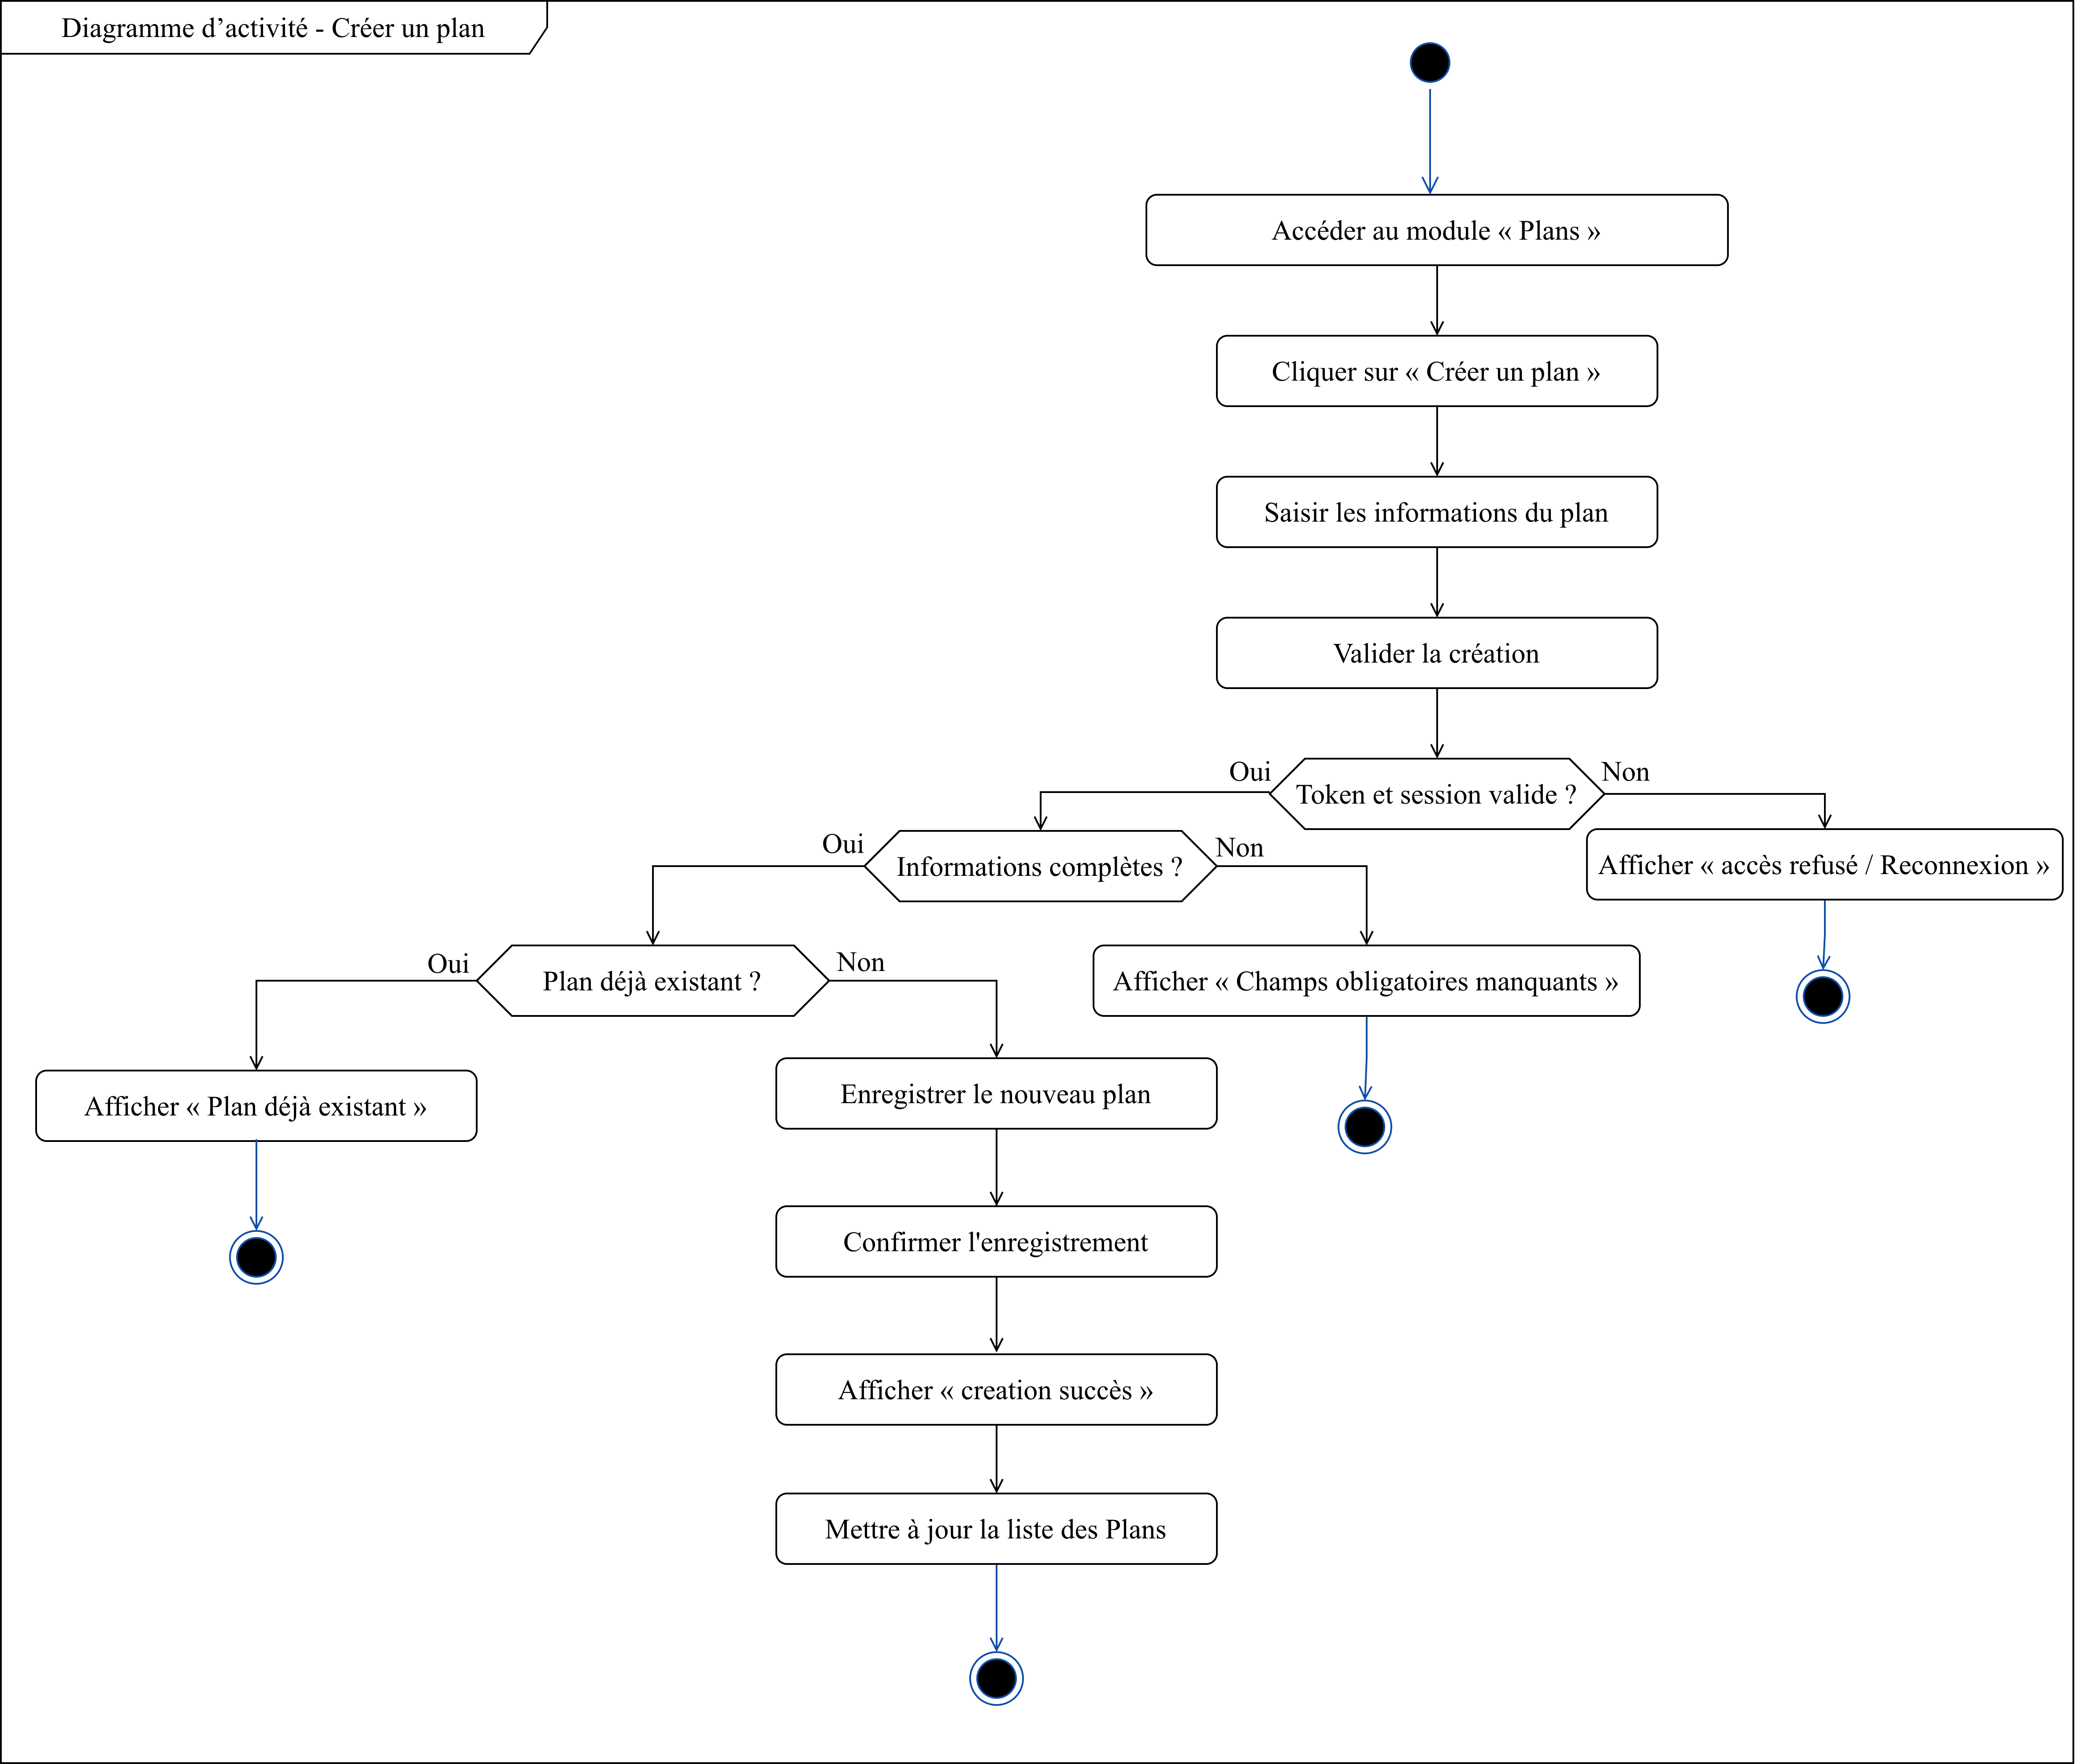
\includegraphics[width=1\linewidth]{figures/chapitre-04/Diagramme_dactivite_cree_un_plan.png}
  \caption{Diagramme d’activité — «~Créer un plan CSR~».}
  \label{fig:doc-ch4-act-creer-plan}
\end{figure}%


\subsubsection{Diagramme d’activité : «~Modifier une activité planifiée~»}

La figure~\ref{fig:doc-ch4-act-modif-activite} présente le diagramme d’activité du cas «~Modifier une activité planifiée~».

\begin{figure}[H]
  \centering
  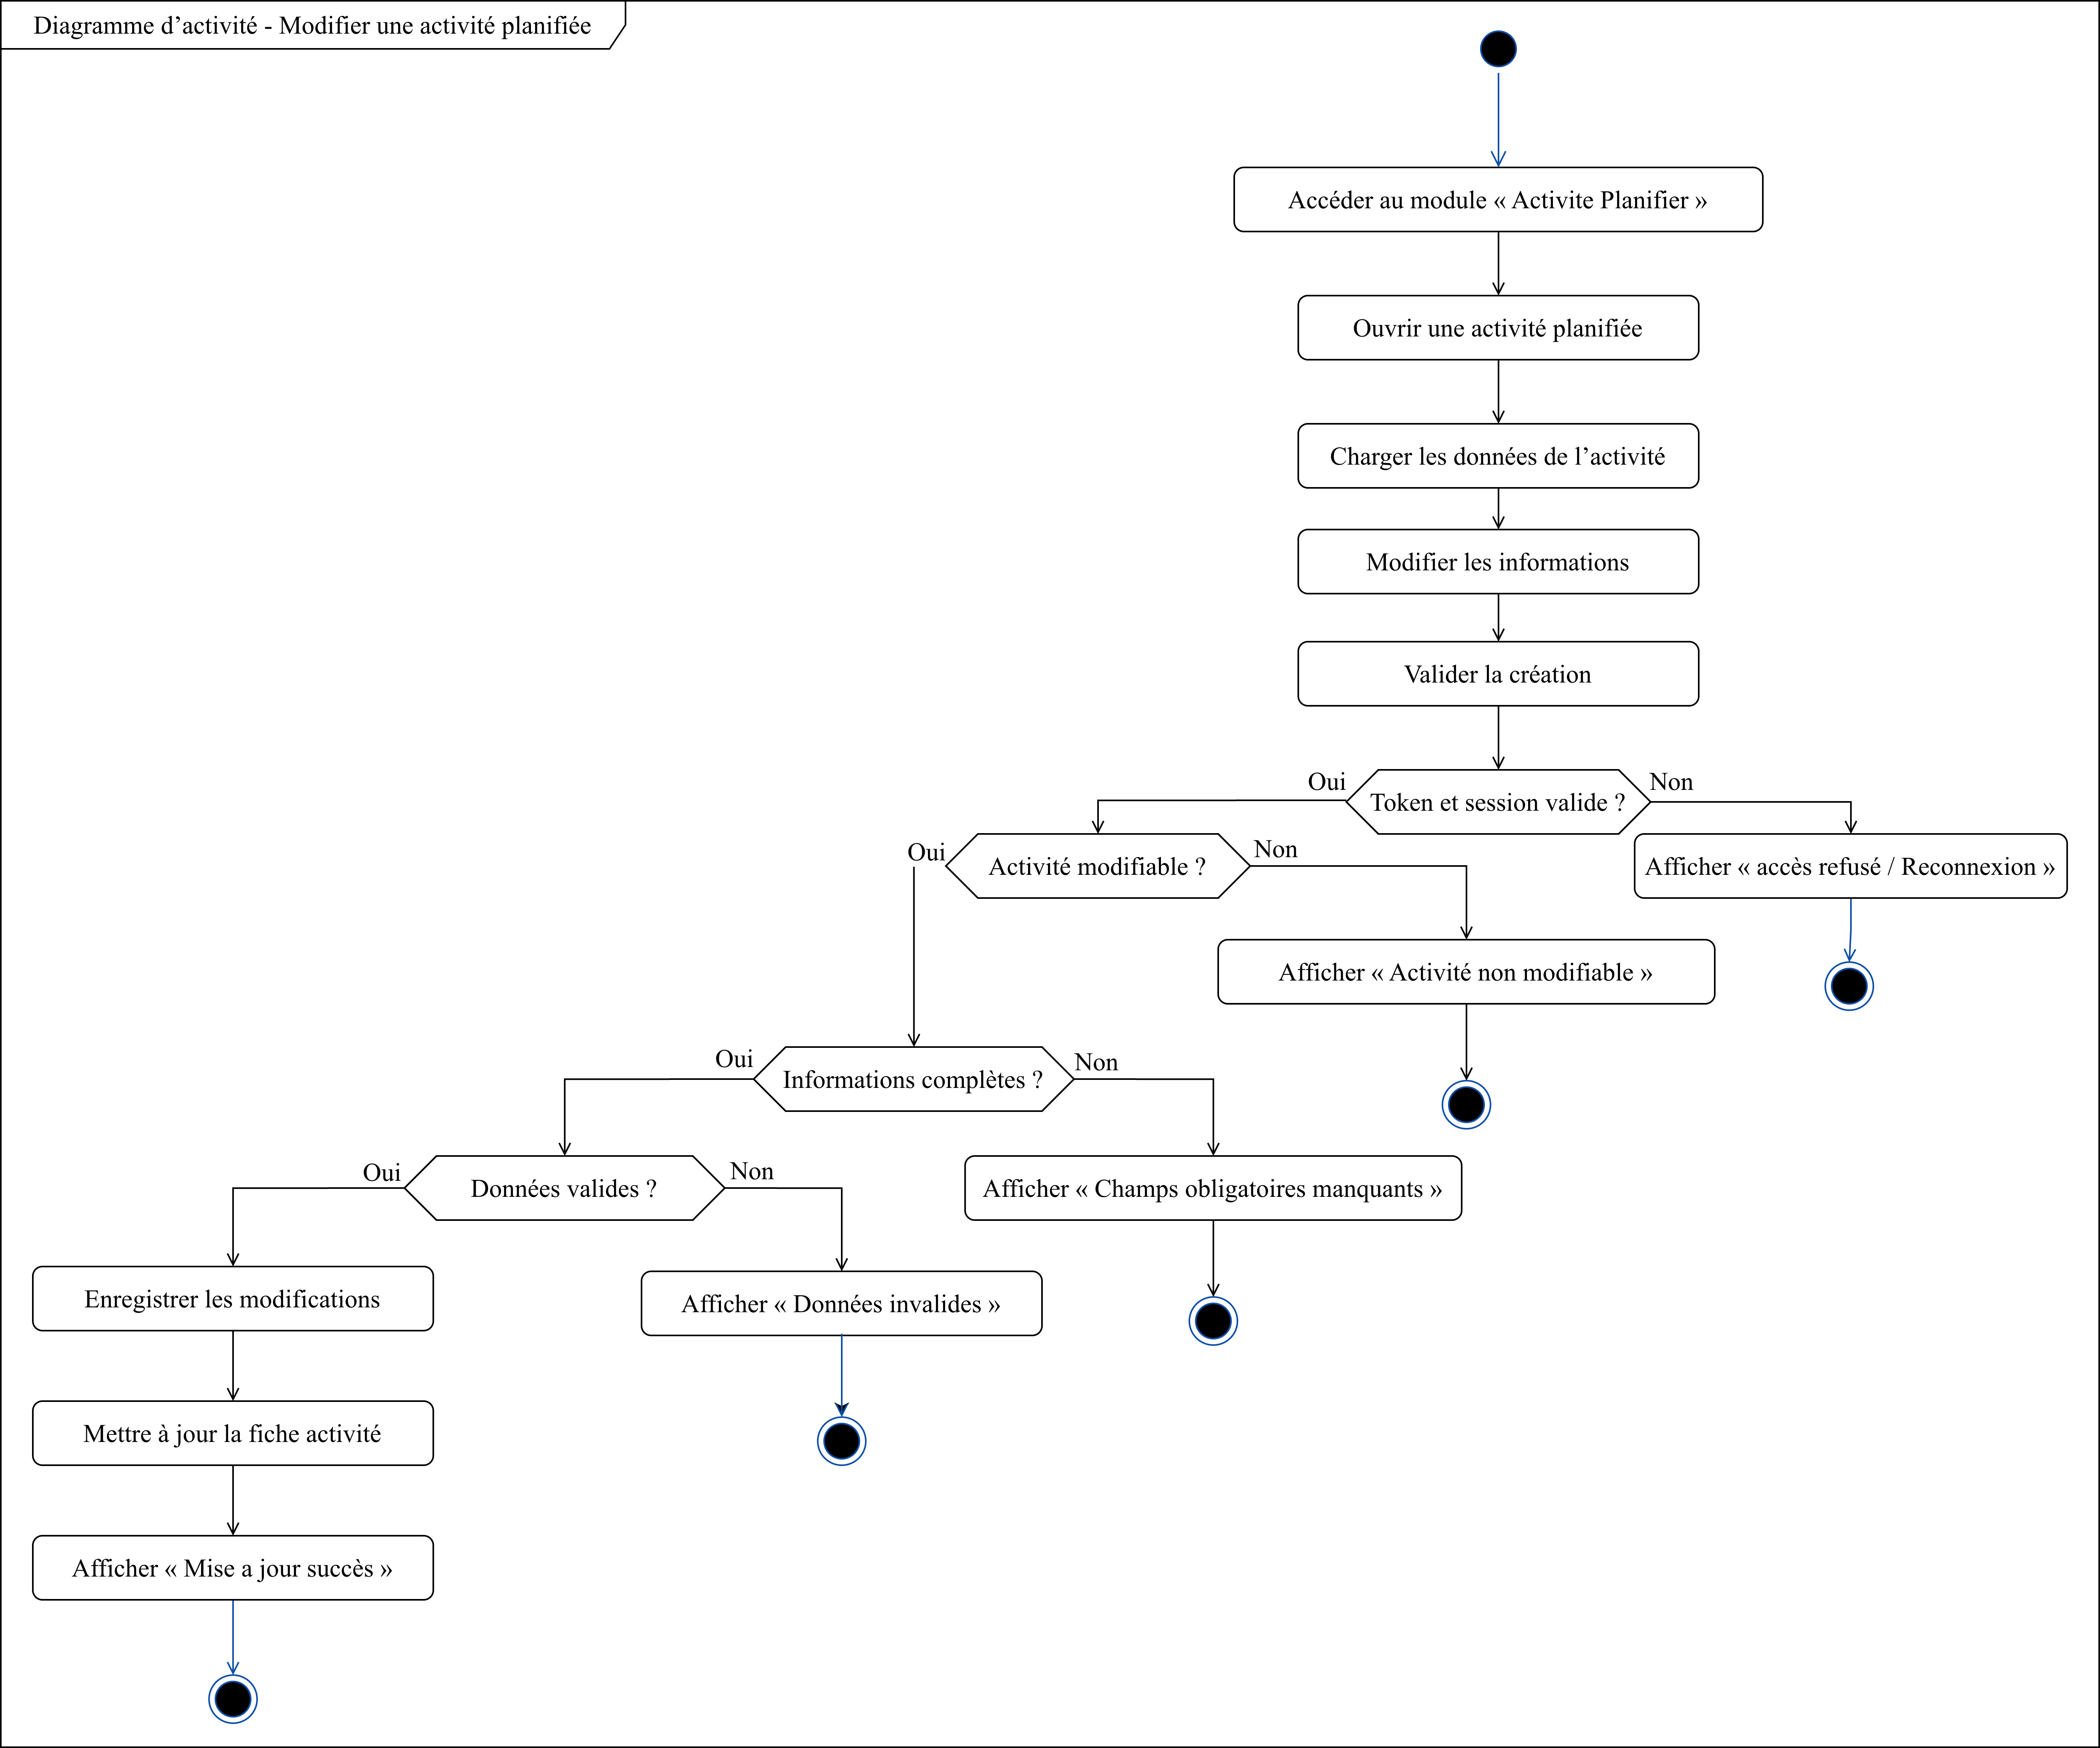
\includegraphics[width=1\linewidth]{figures/chapitre-04/Diagramme_dactivite_modifier_une_activite.png}
  \caption{Diagramme d’activité — «~Modifier une activité planifiée~».}
  \label{fig:doc-ch4-act-modif-activite}
\end{figure}%

\section{Réalisation}

Dans cette section, nous présentons les interfaces réalisées au cours de ce deuxième sprint. Les captures d'écran ci-dessous montrent les principales fonctionnalités développées, notamment la gestion des plans CSR annuels, le suivi des activités planifiées et la saisie des activités réalisées par site. Ces visuels permettent de constater que les fonctionnalités correspondent bien aux besoins définis dans le backlog du sprint.

La figure~\ref{fig:doc-ch4-3} présente la vue liste des plans annuels CSR.

\IfFileExists{figures/chapitre-04/ui-liste-plans-annuels.png}{%
\begin{figure}[H]
  \centering
  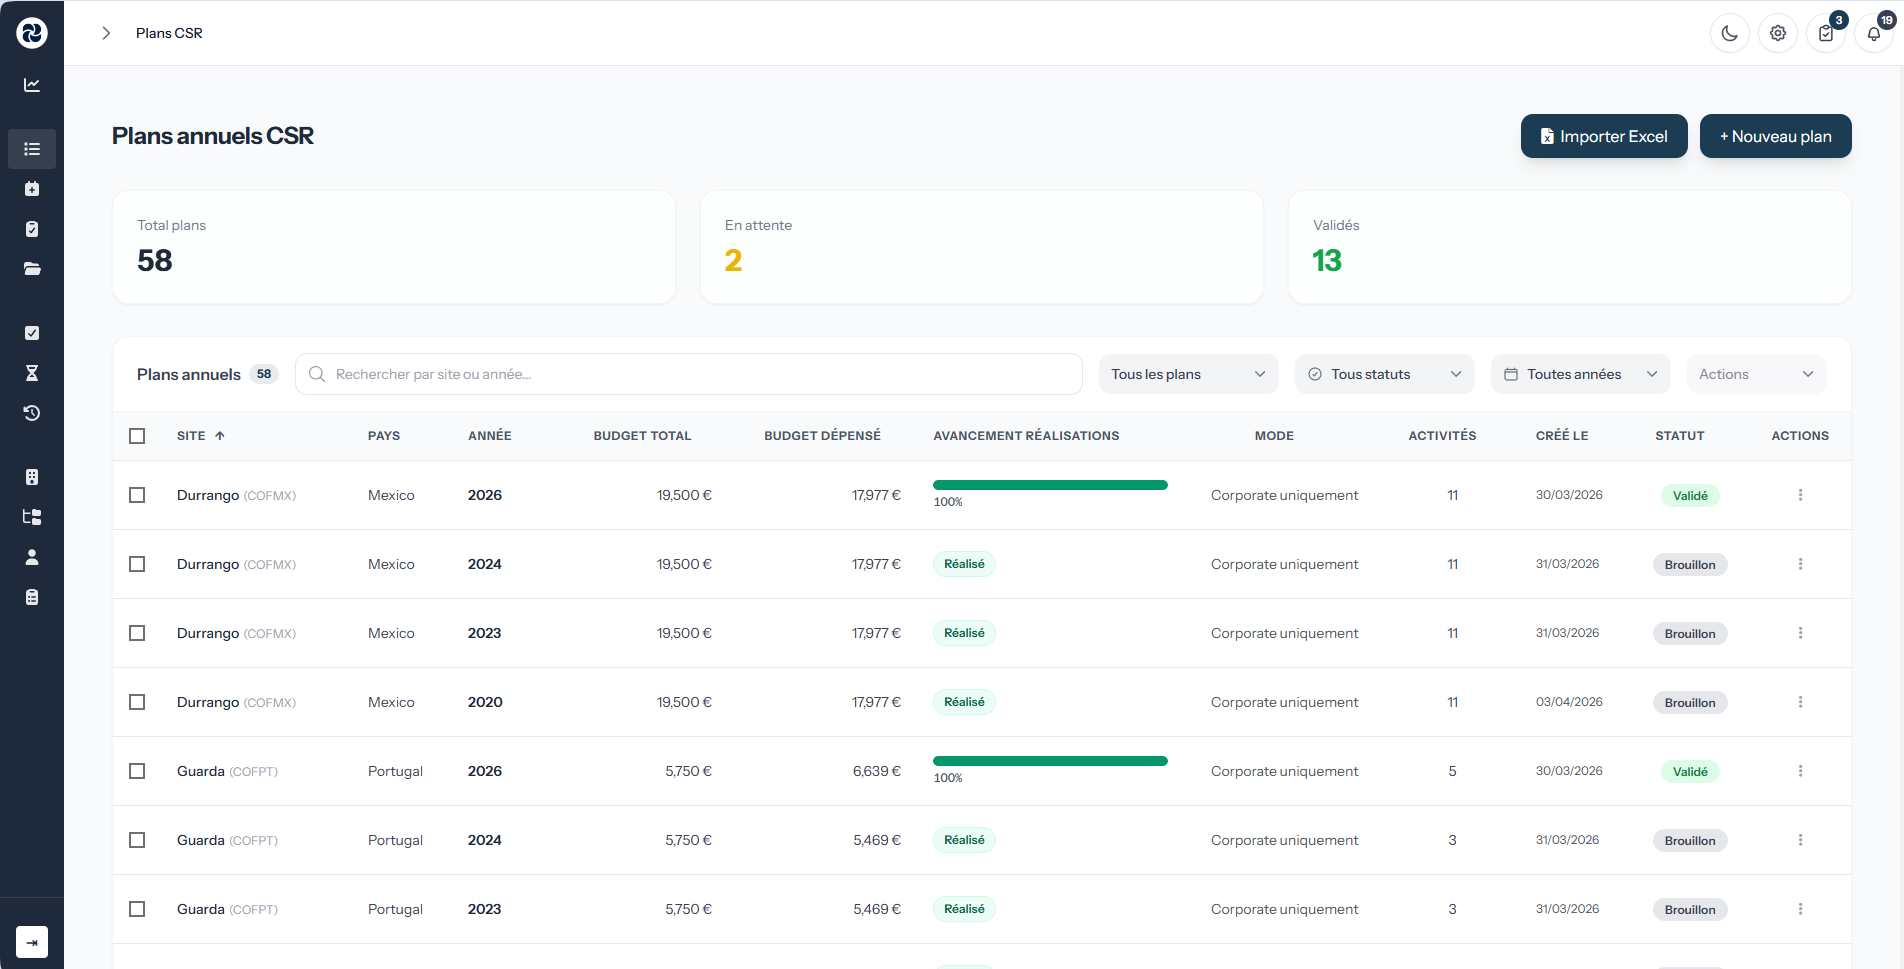
\includegraphics[width=0.92\linewidth]{figures/chapitre-04/ui-liste-plans-annuels.png}
  \caption{Interface : liste des plans annuels CSR.}
  \label{fig:doc-ch4-3}
\end{figure}%
}{%
\begin{figure}[H]
  \centering
  \fbox{\parbox{0.92\linewidth}{\centering\vspace{3.2cm}\textit{(Figure à insérer : \texttt{figures/chapitre-04/ui-liste-plans-annuels.png})}\vspace{3.2cm}}}
  \caption{Interface : liste des plans annuels CSR.}
  \label{fig:doc-ch4-3}
\end{figure}%
}

Cette interface constitue le point d'entrée central du module de planification CSR. Elle offre à l'utilisateur une vue d'ensemble immédiate grâce à trois compteurs affichés en haut de l'écran : le nombre total de plans enregistrés, le nombre de plans en attente de validation et le nombre de plans validés.

Le tableau principal liste les plans par site et par année, en exposant pour chacun le budget total prévu, le budget effectivement dépensé, le taux d'avancement des réalisations sous forme de barre de progression, le mode de validation appliqué, le nombre d'activités rattachées, la date de création ainsi que le statut courant.

Deux actions rapides sont accessibles en haut à droite : la création manuelle d'un nouveau plan et l'import depuis un fichier Excel, couvrant ainsi les deux modes de saisie prévus dans le backlog. Des filtres par site, par statut et par année permettent d'affiner l'affichage selon le besoin de l'utilisateur, qu'il soit responsable d'un seul site ou administrateur corporate supervisant l'ensemble des entités.


\section{Tests et validation}

Les tests occupent une place centrale dans la méthodologie agile, car ils garantissent la qualité ainsi que la fiabilité des fonctionnalités développées. Avant le lancement d’un nouveau sprint, il est indispensable de valider les incréments prioritaires afin de vérifier leur bon fonctionnement et leur conformité aux besoins des parties prenantes.
\subsection{Test}

Dans cette partie, nous présentons une validation fonctionnelle consolidée des fonctionnalités du sprint~2 : gestion des plans CSR, activités planifiées, activités réalisées (y compris hors plan), import Excel et contrôle des doublons.
Le tableau~\ref{tab:ch4-scenarios-tests} synthétise les cas de test correspondants.

% Scénarios de test consolidés — chapitre 4 (plans & activités)
\small
\PFETableSetup
\setlength{\LTpre}{0pt}
\setlength{\LTpost}{0pt}
\setlength{\LTleft}{\fill}
\setlength{\LTright}{\fill}
\setlength{\tabcolsep}{3.5pt}
\renewcommand{\arraystretch}{1.25}

\begin{longtable}{|>{\centering\arraybackslash}m{2.8cm}|
>{\raggedright\arraybackslash}p{2.5cm}|
>{\raggedright\arraybackslash}p{3.8cm}|
>{\raggedright\arraybackslash}p{4.3cm}|
>{\centering\arraybackslash}p{1.1cm}|}
\caption{Synthèse des cas de test du sprint 2}\label{tab:ch4-scenarios-tests}\\
\hline
\tableHeaderStyle
\multicolumn{1}{|c|}{\tableHeaderCell{Nom du cas d'utilisation}} &
\multicolumn{1}{c|}{\tableHeaderCell{Cas de test}} &
\multicolumn{1}{c|}{\tableHeaderCell{Description du cas}} &
\multicolumn{1}{c|}{\tableHeaderCell{Résultat attendu}} &
\multicolumn{1}{c|}{\tableHeaderCell{Résultat réel}} \\
\hline
\endfirsthead
\hline
\multicolumn{5}{|c|}{\tablename\ \thetable{} --- \textit{(suite)}} \\
\hline
\tableHeaderStyle
\multicolumn{1}{|c|}{\tableHeaderCell{Nom du cas d'utilisation}} &
\multicolumn{1}{c|}{\tableHeaderCell{Cas de test}} &
\multicolumn{1}{c|}{\tableHeaderCell{Description du cas}} &
\multicolumn{1}{c|}{\tableHeaderCell{Résultat attendu}} &
\multicolumn{1}{c|}{\tableHeaderCell{Résultat réel}} \\
\hline
\endhead
\hline
\multicolumn{5}{|r|}{\textit{Suite page suivante\ldots}} \\
\hline
\endfoot
\hline
\endlastfoot

\needspace{16\baselineskip}
\multirow{7}{=}{\centering Gérer un plan CSR\\manuellement} &
Créer un plan CSR &
Création d'un nouveau plan annuel avec site, année et budget. &
Le plan est enregistré et visible dans la liste. &
Vrai \\
\cline{2-5}
 &
Consulter un plan CSR &
Ouverture du détail d'un plan déjà créé. &
Les informations du plan sont affichées correctement. &
Vrai \\
\cline{2-5}
 &
Modifier un plan CSR &
Mise à jour des informations d'un plan en état modifiable. &
Les modifications sont enregistrées et visibles. &
Vrai \\
\cline{2-5}
 &
Supprimer un plan CSR &
Suppression d'un plan autorisée selon les règles métier. &
Le plan est supprimé et n'apparaît plus dans la liste. &
Vrai \\
\cline{2-5}
 &
Soumettre un plan CSR pour validation &
Soumission d'un plan complet pour lancer le workflow de validation. &
Le statut passe en « soumis » et le plan devient non modifiable. &
Vrai \\
\cline{2-5}
 &
Importer un plan via Excel &
Import d'un fichier Excel pour créer plan et activités associées. &
Le plan et ses activités sont créés si les données sont valides. &
Vrai \\
\cline{2-5}
 &
Lire et parser le fichier Excel avant l'import &
Vérification de la structure et des données avant confirmation d'import. &
Les erreurs de format sont détectées avant insertion. &
Vrai \\
\hline

\needspace{10\baselineskip}
\multirow{4}{=}{\centering Gérer une activité\\planifiée} &
Créer une activité planifiée &
Ajout d'une nouvelle activité dans un plan CSR. &
L'activité est enregistrée et affichée dans le plan. &
Vrai \\
\cline{2-5}
 &
Consulter une activité planifiée &
Ouverture des détails d'une activité planifiée existante. &
Les informations détaillées sont affichées. &
Vrai \\
\cline{2-5}
 &
Modifier une activité planifiée &
Mise à jour des informations d'une activité planifiée. &
Les modifications sont sauvegardées. &
Vrai \\
\cline{2-5}
 &
Supprimer une activité planifiée &
Suppression d'une activité planifiée selon les règles d'état. &
L'activité est retirée de la liste du plan. &
Vrai \\
\hline

\needspace{10\baselineskip}
\multirow{4}{=}{\centering Gérer une activité\\réalisée} &
Saisir les données réelles de l'activité &
Saisie des données de réalisation (quantités, coûts, période, etc.). &
La réalisation est enregistrée avec succès. &
Vrai \\
\cline{2-5}
 &
Consulter une activité réalisée &
Affichage des détails d'une activité déjà réalisée. &
Les données réelles sont consultables. &
Vrai \\
\cline{2-5}
 &
Modifier une activité réalisée &
Mise à jour des données d'une activité réalisée. &
Les modifications sont enregistrées. &
Vrai \\
\cline{2-5}
 &
Supprimer une activité réalisée &
Suppression d'une réalisation autorisée. &
La réalisation est supprimée de la liste. &
Vrai \\
\hline

\needspace{12\baselineskip}
\multirow{5}{=}{\centering Gérer une activité\\réalisée hors plan} &
Créer une activité réalisée hors plan &
Création d'une activité réalisée non prévue dans le plan initial. &
L'activité hors plan est enregistrée. &
Vrai \\
\cline{2-5}
 &
Consulter une activité réalisée hors plan &
Affichage du détail d'une activité hors plan. &
Les informations sont affichées correctement. &
Vrai \\
\cline{2-5}
 &
Modifier une activité réalisée hors plan &
Mise à jour des informations d'une activité hors plan. &
Les modifications sont sauvegardées. &
Vrai \\
\cline{2-5}
 &
Supprimer une activité réalisée hors plan &
Suppression d'une activité hors plan existante. &
L'activité est supprimée de la liste. &
Vrai \\
\cline{2-5}
 &
Soumettre une activité réalisée hors plan pour validation &
Envoi de l'activité hors plan dans le circuit de validation. &
Le statut passe en attente de validation. &
Vrai \\
\hline

\needspace{7\baselineskip}
\multirow{2}{=}{\centering Contrôler les\\duplicatas (import Excel)} &
Supprimer les duplicatas &
Suppression des lignes dupliquées avant import. &
Les doublons sont retirés du jeu de données. &
Vrai \\
\cline{2-5}
 &
Ignorer les duplicatas et continuer &
Poursuite de l'import en ignorant les lignes dupliquées détectées. &
L'import continue sans bloquer sur les doublons. &
Vrai \\
\hline

\end{longtable}
\normalsize


\newpage

Les figures~\ref{fig:ch4-postman-plans} sont prévues pour les captures correspondantes.

\begin{figure}[H]
  \centering
  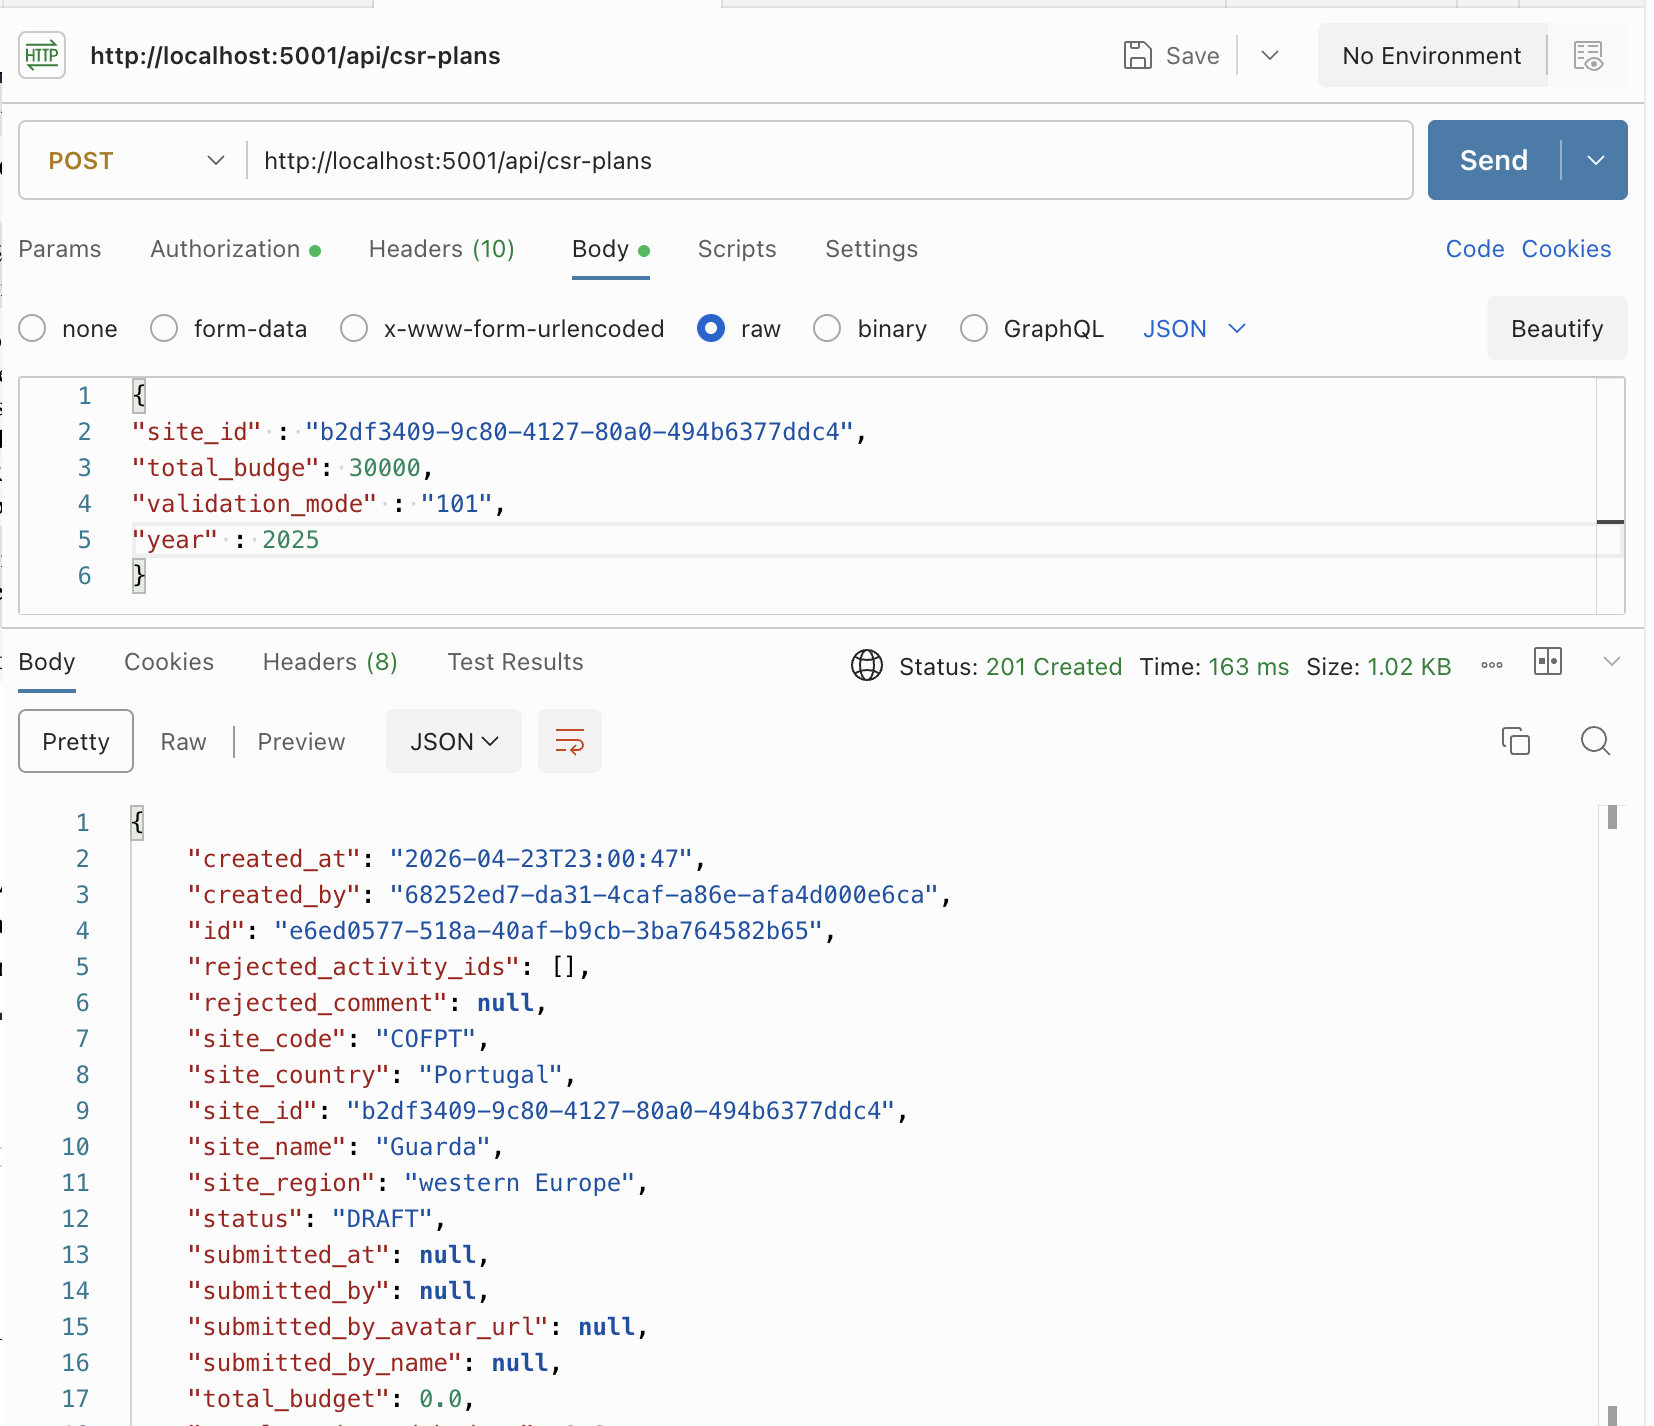
\includegraphics[width=0.92\linewidth]{figures/chapitre-04/postman-csr-plans.png}
  \caption{Tests Postman — création de plan.}
  \label{fig:ch4-postman-plans}
\end{figure}

\subsection{Validation}

Une revue de fin de sprint avec le \emph{Scrum Master} et le \emph{Product Owner} a permis de valider les parcours plans et activités CSR (création, importation, modification, suppression). Les correctifs mineurs d'ergonomie et de messages utilisateur ont été intégrés avant la bascule vers le sprint suivant centré sur les workflows transverses.

\section{Conclusion}

Ce sprint enrichit la plateforme en couvrant le cœur métier de la planification CSR par site et en préparant le terrain pour le suivi de l'exécution.

Il ouvre la voie au sprint suivant, dédié aux workflows transverses (validations croisées, demandes de modification, notifications et traçabilité).
